\documentclass[lettersize,journal]{IEEEtran}
\usepackage{amsmath,amsfonts,amssymb}
\usepackage{algorithmic}
\usepackage{algorithm}
\usepackage{array}
\usepackage[caption=false,font=normalsize,labelfont=sf,textfont=sf]{subfig}
\usepackage{textcomp}
\usepackage{stfloats}
\usepackage{url}
\usepackage{verbatim}
\usepackage{graphicx}
\usepackage{cite}
\usepackage{multirow}
\usepackage{booktabs}
\usepackage{threeparttable}
\usepackage{enumitem}
\hyphenation{op-tical net-works semi-conduc-tor IEEE-Xplore}
% updated with editorial comments 8/9/2021


\usepackage{orcidlink}


\begin{document}

\title{Graph Learning for Topology-Adaptive Fast Frequency Response in Inverter-Based Microgrids}

% \author{IEEE Publication Technology,~\IEEEmembership{Staff,~IEEE,}
%         % <-this % stops a space
% \thanks{This paper was produced by the IEEE Publication Technology Group. They are in Piscataway, NJ.}% <-this % stops a space
% \thanks{Manuscript received April 19, 2021; revised August 16, 2021.}}

\author{Tran Kim Nhat, Nguyen Van Cuong\orcidlink{0000-0001-8877-7735},~\IEEEmembership{Graduate Student Member,~IEEE}, Nguyen Phi Long\orcidlink{0000-0002-3788-8731},~\IEEEmembership{Member,~IEEE}, and Laurent El Ghaoui\orcidlink{0000-0002-0499-5610}
	
%	\thanks{Manuscript received January 1, 20xx; revised xxxx xx, xxxx. \textit{(Corresponding author: Nguyen Phi Long)}. The authors acknowledge the financial support provided by the Vingroup Innovation Foundation (VINIF) under Project VINIF.2025.DA119.}
	
	\thanks{The authors acknowledge the financial support provided by the Vingroup Innovation Foundation (VINIF) under Project VINIF.2025.DA119. \textit{(Corresponding author: Nguyen Phi Long.)}}
		
	\thanks{T.K. Nhat, N.V. Cuong, N.P. Long, and Laurent El Ghaoui, are with Center for Environmental Intelligence and College of Engineering \& Computer Science, VinUniversity, Hanoi 100000, Vietnam (e-mail: nhat.tk@vinuni.edu.vn; 25cuong.nv@vinuni.edu.vn; long.np2@vinuni.edu.vn; laurent.eg@vinuni.edu.vn).}
	
	\thanks{N.V. Cuong and N.P. Long are also with School of Electrical and Electronic Engineering, Hanoi University of Industry, Hanoi 100000, Vietnam (e-mail: cuongnv@haui.edu.vn; long.nguyen04@haui.edu.vn).}
}



% The paper headers
% \markboth{Journal of \LaTeX\ Class Files,~Vol.~14, No.~8, August~2021}%
% {Shell \MakeLowercase{\textit{et al.}}: A Sample Article Using IEEEtran.cls for IEEE Journals}

%\IEEEpubid{0000--0000/00\$00.00~\copyright~2021 IEEE}
% Remember, if you use this you must call \IEEEpubidadjcol in the second
% column for its text to clear the IEEEpubid mark.

\maketitle

\begin{abstract}
High penetration of inverter-based resources (IBRs) in islanded microgrids reduces system inertia, threatening frequency stability under topology changes. This paper proposes a topology-adaptive fast frequency response (FFR) controller that couples an inductive GraphSAGE encoder with a parameter-shared multi-agent proximal policy optimization (MAPPO) actor. Controllable distributed energy resources (DERs) jointly optimize active-power references and local droop gains under a centralized training with decentralized execution framework. To capture structural grid variations, the training environment incorporates a topology-dependent reduced state-space frequency model via Kron reduction. Frequency security is strictly guaranteed by structural stability through a monotone droop parameterization with a Lyapunov certificate and a closed-form nadir-projection safety layer. Validated under a zero-shot topology hold-out on a modified IEEE 123-bus feeder---held-out configurations differing from the nearest training topology by a Jaccard edge distance up to $\approx\!0.18$, an order of magnitude beyond a random-reconfiguration split, though still bounded by the radial feeder's reachable configurations---the controller reduces the post-event integral absolute frequency error (IAE) by 58\%–75\% and improves the frequency nadir by up to 0.74 Hz compared to classical fixed droop.
\end{abstract}



\begin{IEEEkeywords}
Fast frequency response (FFR), islanded microgrids (IMGs), inverter-based resources (IBR), virtual power plant (VPP), GraphSAGE network, multi-agent reinforcement learning (MARL), proximal policy optimization (PPO)
\end{IEEEkeywords}

% =====================================================================
\section*{Nomenclature}
\addcontentsline{toc}{section}{Nomenclature}
\begin{IEEEdescription}[\IEEEsetlabelwidth{$\Delta\boldsymbol{\delta}_{\mathrm{rel}}$}]

\item[\emph{Indices and Sets}]\hfill
\item[$g,\,i,\,m$] Index of GFM unit, DER, and learning agent.
\item[$t,\,z,\,k,\,h$] Index of time step, VPP zone, GNN layer, harmonic.
\item[$I,\,L$] Retained GFM buses; eliminated load buses.
\item[$\mathcal{A},\,\mathcal{A}_z$] Set of GFL agents; agents of zone $z$.
\item[$\mathcal{Z}$] Set of VPP zones.
\item[$\mathcal{G}_t$] Active feeder graph at step $t$.
\item[$\mathcal{N}(j)$] One-hop neighborhood of node $j$ on $\mathcal{G}_t$.

\item[\emph{Parameters and Constants}]\hfill
\item[$H_g,\,H_{\mathrm{sys}}$] GFM virtual inertia; aggregate system inertia.
\item[$D_g$] GFM damping coefficient.
\item[$f_0,\,\omega_0$] Nominal frequency; $\omega_0=2\pi f_0$.
\item[$S_{\mathrm{base}},\,S_g$] System base power; rating of unit $g$.
\item[$n_g$] Number of GFM units.
\item[$\eta_{\mathrm{ch}},\eta_{\mathrm{dis}}$] Charge/discharge efficiency.
\item[$E,\,P_{\mathrm{rated}}$] Energy capacity; rated power of a DER.
\item[$\Delta t,\,\Delta T$] Fast control step; dispatch interval.
\item[$K_{\min},K_{\max}$] Lower/upper droop-gain bound.
\item[$k_{\mathrm{agc}}$] Secondary (AGC) loop gain.
\item[$\delta$] Nadir-admissible COI band ($0.5$\,Hz).
\item[$\gamma,\,\lambda,\,\epsilon$] Discount; GAE factor; PPO clip range.

\item[\emph{Variables}]\hfill
\item[$\Delta\omega_g,\Delta\delta_g$] Per-unit frequency/angle deviation of unit $g$.
\item[$\Delta\boldsymbol{\delta}_{\mathrm{rel}},\Delta\boldsymbol{\omega}$] Relative-angle and frequency-deviation vectors.
\item[$x,\,u_t$] State vector; control input.
\item[$\Delta P_{\mathrm{set},g},\Delta P_{e,g}$] Power set point; electrical-power deviation.
\item[$\Delta P_{\mathrm{ref}},\Delta P_{\mathrm{imb}}$] Commanded reference; disturbance imbalance.
\item[$\Delta P^{\mathrm{ffr}}_{i,t}$] Incremental FFR power of DER $i$.
\item[$R^{\mathrm{ffr}}_{i,t}$] Deliverable FFR reserve of DER $i$.
\item[$\mathrm{SoC}_t$] State of charge.
\item[$V_t,\,S_t$] Bus-voltage profile; inverter apparent-power loading.
\item[$P_t,\,Q_t$] Active/reactive line-flow vectors.
\item[$\Delta f_t,\,\dot f_t$] COI frequency deviation; RoCoF.
\item[$\zeta_t$] Secondary-loop integral state.
\item[$a_m,a^P_m,a^K_m$] Agent action; power and droop channels.
\item[$K_m$] Learned local droop gain of agent $m$.
\item[$H_j^{(k)}$] Embedding of node $j$ at GraphSAGE layer $k$.
\item[$r_t,\,\hat A_t,\,\rho_t$] Team reward; GAE advantage; PPO ratio.

\item[\emph{Matrices, Functions, and Operators}]\hfill
\item[$A_f(\mathcal{G}_t,K_t)$] Topology-parameterized state matrix.
\item[$B_{\mathrm{ref}},B_{\mathrm{net}}$] Reference and located-disturbance input maps.
\item[$\tilde J_r,\,J_{(\cdot)}$] Kron-reduced active-power Jacobian and blocks.
\item[$D(K_t)$] Effective damping matrix.
\item[$\Phi,\,\Gamma$] Discrete-time (ZOH) state/input matrices.
\item[$W_{\mathrm{self}},W_{\mathrm{neigh}}$] Shared GraphSAGE aggregator weights.
\item[$\mathcal{L}^{\mathrm{clip}}$] Clipped PPO surrogate loss.
\item[$V,\,M,\,\mathbf P$] Lyapunov function; inertia matrix; LMI certificate.

\item[\emph{Abbreviations}]\hfill
\item[FFR / IBR] Fast frequency response / inverter-based resource.
\item[GFM / GFL] Grid-forming / grid-following.
\item[VSG / VPP] Virtual synchronous generator / virtual power plant.
\item[DER / DSO] Distributed energy resource / distribution-system operator.
\item[BESS / V2G] Battery storage / vehicle-to-grid; DPV: distributed PV.
\item[MARL / MAPPO] Multi-agent RL / multi-agent PPO.
\item[CTDE] Centralized training, decentralized execution.
\item[COI / RoCoF] Center of inertia / rate of change of frequency.
\item[UFLS / DLMP] Underfrequency load shedding / distribution LMP.
\item[IAE / ITAE] Integral (time-weighted) absolute frequency error.
\item[THD / SoC] Total harmonic distortion / state of charge.

\end{IEEEdescription}

\section{Introduction}
% ==================================================================
\label{sec:intro}
% ==================================================================

% ------------------------------------------------------------------
%  I-A  Background and Motivation
% ------------------------------------------------------------------
\subsection{Background and Motivation}
\label{ssec:background}

\IEEEPARstart{T}{he} transition toward $100$\,\% inverter-based resources (IBRs) in islanded distribution feeders displaces the rotating synchronous generators that have traditionally supplied inertia and primary frequency support. The resulting reduction in system inertia raises the rate of change of frequency (RoCoF) after a power imbalance event and pushes the post-disturbance frequency \emph{nadir} closer to under frequency load shedding (UFLS) thresholds; in low-inertia islanded systems, both effects together can trigger UFLS stages and, in severe cases, cascading generator trips that lead to a complete blackout~\cite{shobug2024vicreview,roy2022overview,khayat2021virtual}. Restoring secure frequency operation under these conditions requires the inverter-interfaced distributed energy resources (DERs) themselves battery energy storage (BESS), vehicle-to-grid (V2G) chargers, and distributed photovoltaics (DPV) to deliver \emph{fast frequency response} (FFR) on millisecond second time scales, in coordination with grid-forming (GFM) inverters that establish the voltage and frequency reference~\cite{lin2022field,bakeer2024bidirectional,perez2023adaptive,salem2025gfmreview}.

The dominant FFR scheme in deployed islanded microgrids today is the \emph{classical droop} controller, in which every DER emits an incremental active-power response


\begin{equation}
\Delta P^{\mathrm{ffr}}_{i,t}=-K_i\,\Delta f_t
\label{eq:classical_droop}
\end{equation}


proportional to the local frequency deviation, with a fixed per-device gain~$K_i$. Although effective near a single operating point, the classical droop loop has two structural limitations that this paper aims to remove.

\emph{First, the gain is fixed.} The gain~$K_i$ is set at commissioning to a value that is conservative for the worst foreseeable disturbance, so the droop response is systematically under-utilized during mild events and offers no mechanism to amplify the gain under near-UFLS conditions or to surrender headroom when storage energy is scarce. Adaptive virtual-inertia and adaptive-VSG controllers improve on this trade-off but typically tune~$K_i$ through a small-signal model evaluated around a fixed operating point~\cite{boutfarjoute2025fuzzy,kerdphol2017robust,saxena2020derivative}.

\emph{Second, the controller is topology-blind.} The deliverability of an FFR commitment in an islanded feeder is not a property of the DER fleet alone; it is jointly determined by the \emph{active feeder topology}, because tie-switch reconfiguration performed by the distribution-system operator (DSO) and unplanned line contingencies alter the electrical paths between DER buses and the GFM reference~\cite{mohyuddin2022dsovpp,jacob2024outage}. The same per-DER
droop gain therefore produces markedly different transient frequency responses depending on which buses remain electrically connected to the GFM reference, yet neither the gain~$K_i$ nor the controller's internal state  representation in \eqref{eq:classical_droop} encode the active graph in any way.

Multi-agent reinforcement learning (MARL) controllers improve the gain-adaptation issue but inherit the topology-blindness issue. Existing MARL FFR controllers based on multi-layer-perceptron (MLP) encoders or transductive graph convolutions embed a \emph{fixed} adjacency matrix during training~\cite{wang2025mappo,qiu2023hierarchical,wang2023graphppo,guo2024gcnnppo,guo2024ldlfc,shi2025coordvpp}, so the agents' observations, message-passing neighborhoods, and learned policies are all tied to the training graph and degrade under tie-switch reconfiguration and line contingencies. Inductive graph neural networks such as GraphSAGE~\cite{hamilton2017graphsage} learn aggregator functions that generalize to unseen graphs and have recently been applied to topology-varying emergency control ~\cite{pei2023graphsage} for undervoltage load shedding on transmission systems. To the best of our knowledge, however, inductive graph encoders have not previously been combined with cooperative MARL to \emph{replace} the classical droop loop for FFR delivery in $100$\,\% IBR islanded microgrids, nor evaluated under a zero-shot topology hold-out protocol on frequency-security metrics.

This paper closes that gap by developing a topology-adaptive GraphSAGE--MAPPO controller in which (i)~each DER simultaneously emits a fast active-power reference and a local droop gain, replacing the fixed-gain response of~\eqref{eq:classical_droop} with a learned, state-conditioned response, and (ii)~the policy reasons over the active feeder graph through an inductive GraphSAGE encoder so that the same controller transfers without retraining to unseen feeder configurations.

% ------------------------------------------------------------------
%  I-B  Literature Review
% ------------------------------------------------------------------
\subsection{Literature Review}
\label{ssec:litreview}

\subsubsection{Virtual-inertia and VSG control for islanded microgrids}

A large body of work studies FFR in islanded microgrids through virtual-synchronous-generator (VSG), droop, virtual-inertia, and related controllers. Adaptive VSG and fuzzy- or metaheuristic-tuned virtual-inertia controllers improve RoCoF and frequency nadir compared with fixed-droop schemes under time-varying renewable generation~\cite{boutfarjoute2025fuzzy, hamanah2024robust,mishra2024metaheuristic}, and recent reviews and field demonstrations confirm that GFM--VSG inverters can stabilize frequency in $100$\,\% IBR microgrids without rotating machines ~\cite{perez2023adaptive,bakeer2024bidirectional,salem2025gfmreview,sati2025economic}. Nevertheless, almost all of these studies tune the controller on a fixed feeder topology and around a fixed operating point; the inertia and damping coefficients are re-optimized through small-signal analysis whenever the operating point changes, and topology variation is treated, at most, as parametric uncertainty rather than as a structural change in the underlying graph~\cite{mishra2024metaheuristic,hamanah2024robust}.

\subsubsection{MARL for frequency control in microgrids}

MARL has emerged as a scalable approach for coordinating large populations of inverter-interfaced DERs to provide FFR under centralized training with decentralized execution (CTDE)~\cite{dolatyabi2025happo,shi2025coordvpp}. Standard MAPPO, MADDPG, and MASAC formulations demonstrate effective economic dispatch, voltage regulation, and primary frequency control, but they typically use either MLP encoders or graph-convolutional encoders that embed a fixed adjacency matrix~\cite{wang2025mappo,qiu2023hierarchical,wang2023graphppo,guo2024gcnnppo,guo2024ldlfc}. Such controllers are topology-blind: the agents' observation, message-passing neighborhoods, and learned policies are all defined on the training graph, so they do not extend without retraining to feeder configurations not seen during training. Moreover, existing RL-based FFR controllers typically expose either a power-reference action \emph{or} a droop-gain action to the policy but rarely both~\cite{hu2022multitimescale,wang2025mappo}, so the implicit gain reservation is fixed during real-time execution and cannot adapt to the realized topology or to the available storage energy.

\subsubsection{Graph neural networks for power-system control}

This is the body of prior work most closely related to the present paper. Graph neural networks (GNNs) provide an attractive inductive bias for power systems because the grid is naturally a graph, and recent surveys catalogue applications to optimal power flow, state estimation, voltage control, and load-frequency control~\cite{liao2021gnn,liu2022topology}. Within RL-based control, three patterns dominate.
First, \emph{transductive} graph convolutions on a fixed adjacency, e.g., Graph-PPO ~\cite{wang2023graphppo} for distribution-level voltage regulation and GCNN-PPO ~\cite{guo2024gcnnppo} or SGAC ~\cite{guo2024ldlfc} for islanded load-frequency control.
Second, \emph{physics-guided} GNNs that adapt to topology variation through re-training or online transfer, including topology-aware GNN-OPF and PG-GNN ~\cite{liu2022topology,yang2024pggnn}.
Third, \emph{inductive} GNNs aimed at zero-shot transfer to unseen graphs, including the foundational GraphSAGE work~\cite{hamilton2017graphsage}, GraphSAGE-based fault diagnosis and state estimation ~\cite{CHEN2023930}, and closest to the present problem formulation the GraphSAGE-D3QN emergency-control framework of ~\cite{pei2023graphsage}, which uses inductive neighborhood aggregation to adapt undervoltage load-shedding policies to topology variations on the IEEE 39- and 300-bus transmission systems.

The combination of an inductive GraphSAGE encoder with a cooperative on-policy MAPPO actor~\cite{yu2022mappoeffective}, applied
to \emph{FFR control as a replacement for the classical droop loop} in $100$\,\% IBR islanded microgrids, has not, to our knowledge, been investigated. Equally important, existing GraphSAGE power papers~\cite{pei2023graphsage} typically do not adopt a zero-shot topology hold-out evaluation protocol with disjoint training/testing topology sets, and they do not measure the generalization gap on frequency-security metrics (post-event integral absolute frequency error, frequency nadir, maximum RoCoF, FFR success rate against UFLS bounds). We therefore explicitly disclaim novelty of GraphSAGE itself and of the GraphSAGE RL combination~\cite{pei2023graphsage}; our contribution lies in the \emph{problem} (FFR in $100$\,\% IBR islanded microgrids), the \emph{architecture} (per-DER joint power reference/droop gain action sharing one inductive encoder), and the \emph{evaluation} (zero-shot topology hold-out on frequency-security metrics, with the achieved Jaccard edge-distance range reported rather than asserted).

% ------------------------------------------------------------------
%  I-C  Research Gaps
% ------------------------------------------------------------------
\subsection{Research Gaps}
\label{ssec:gaps}

The literature surveyed above motivates three concrete gaps, summarized in Table~\ref{tab:litreview}.
\paragraph*{Gap~1 -- Topology-dependent FFR deliverability is under-modeled}

Most FFR scheduling models compute the available reserve
$R^{\mathrm{ffr}}_{i,t}$ for DER $i$ at time~$t$ as a function of the
local energy state alone:
\begin{equation}
R^{\mathrm{ffr}}_{i,t}\neq f\!\left(\mathrm{SoC}_{i,t}\ \text{only}\right).
\label{eq:gap1bad}
\end{equation}
However, in islanded inverter-based microgrids the deliverability of FFR also depends on the active feeder graph and on the resulting voltage and current envelopes:
\begin{equation}
R^{\mathrm{ffr}}_{i,t}=f\!\left(\mathcal{G}_t,\ \mathrm{SoC}_{i,t},\
V_t,\ S_t,\ P_t,\ Q_t\right),
\label{eq:gap1good}
\end{equation}
where $\mathcal{G}_t$ denotes the active feeder graph, $V_t$ the bus-voltage profile, $S_t$ the inverter apparent-power loading, and $(P_t,Q_t)$ the line-flow vector. Controllers that ignore $\mathcal{G}_t$ commit a reserve that cannot in practice be delivered under the realized topology, producing under-supply and larger frequency excursions.

\paragraph*{Gap~2 -- MARL FFR controllers are not evaluated under a topology hold-out protocol}

A growing literature reports MARL and GNN-MARL controllers for microgrid frequency and voltage control. Evaluation, however, almost universally reuses topologies seen during training, i.e.,
$\mathcal{G}_{\text{train}}\cap\mathcal{G}_{\text{test}}\neq\emptyset$.
A more demanding protocol partitions topologies into disjoint sets,
\begin{equation}
\mathcal{G}_{\text{train}}\cap\mathcal{G}_{\text{test}}=\emptyset,
\label{eq:gap2}
\end{equation}
and reports the resulting zero-shot generalization gap on frequency-security metrics. Outside GraphSAGE-D3QN ~\cite{pei2023graphsage} and a handful of GNN-OPF studies~\cite{yang2024pggnn,liu2022topology}, this protocol is rarely applied to RL-based FFR controllers, and almost never reported on the metrics that matter most for low-inertia microgrid frequency security: post-event integral absolute frequency error (IAE), frequency nadir, maximum RoCoF, and FFR success rate against UFLS bounds.

\paragraph*{Gap~3 -- The active-power reference and the droop gain are exposed separately, never jointly}

In existing MARL FFR formulations, the policy emits either an active-power reference action \emph{or} a droop-gain action, but not both simultaneously. The implicit gain reservation is therefore fixed during real-time execution and cannot trade off transient frequency support against storage energy headroom or service-quality constraints (state-of-charge band). Conversely, when only the droop gain is exposed, the policy cannot pre-position storage assets ahead of an anticipated FFR call. The structural limitation of \eqref{eq:classical_droop} a fixed-gain, scalar response is inherited by these formulations. The present paper exposes both actions to the policy and learns to co-optimize them within a single cooperative Dec-POMDP.

% ------------------------------------------------------------------
%  I-D  Contributions
% ------------------------------------------------------------------
\subsection{Contributions}
\label{ssec:contrib}

Addressing these gaps, this paper makes the
following contributions.

\begin{enumerate}[leftmargin=*]

  \item \textbf{Topology-coupled FFR-deliverability model.}
        We establish that the available FFR reserve and the effectiveness of a per-DER droop commitment are functions of the active feeder graph $\mathcal{G}_t$, the bus-voltage profile~$V_t$, and the inverter apparent-power loading~$S_t$, as in~\eqref{eq:gap1good} a dependency neglected in existing VSG, virtual-inertia, and RL-based FFR controllers. The deliverability model is embedded in a three-layer execution architecture tailored to 100\% IBR islanded operation: the DSO layer clears a second-order-cone optimal power flow with feeder reconfiguration and produces distribution locational marginal prices (DLMP) decomposed into energy, loss, congestion, and voltage components \cite{bai2018dlmp,basdomenech2024dlmp}; Layer~1 (VPP aggregator) solves a Wasserstein distributionally-robust energy-and-reserve bid against price and renewable-output scenarios \cite{liu2021wdrovpp,arrigo2021wdroreserve}; and Layer~2 (GraphSAGE--MAPPO) executes the fast FFR response. The two upper layers are solved day-ahead/offline over a 365-day horizon, and the real-time Layer-2 controller dispatches against the resulting prices as a \emph{price taker}---the standard hierarchical decomposition in which the DSO posts DLMP and aggregators respond, which is provably consistent with the centralized clearing \cite{huang2015dlmp,li2014dlmp,rahimiyan2016pricetaker}. We do not co-optimize real-time delivery with in-horizon re-clearing (no price impact), which is the conventional and appropriate assumption for a distribution-scale price-taking VPP. Crucially, the training environment evaluates the response through a \emph{topology-dependent} reduced state-space frequency model $\mathbf{A}_f(G_t,\mathbf{K}_t)$ in~\eqref{eq:af_matrix}, in which each reconfiguration
        reshapes the inter-GFM coupling through the Kron-reduced network Jacobian, removing the internal inconsistency of driving a \emph{topology-adaptive} policy with a scalar centre-of-inertia model whose parameters are invariant to reconfiguration.

  \item \textbf{GraphSAGE--MAPPO that replaces the classical controller.}
        We develop a cooperative MARL execution policy that pairs an inductive GraphSAGE encoder~\cite{hamilton2017graphsage,pei2023graphsage} with multi-agent PPO~\cite{yu2022mappoeffective} under CTDE. The key design choices are (i)~a parameter-shared actor that emits, for every DER, a two-dimensional action $(a^{P}_{i,t},a^{K}_{i,t})$ jointly setting the fast active-power reference and the local droop gain thereby \emph{replacing} the fixed-gain droop response $\Delta P^{\mathrm{ffr}}_{i,t}=-K_i\,\Delta f_t$ of~\eqref{eq:classical_droop} with a learned, state-conditioned response; (ii)~an agent-centered critic with global mean--max pooling
        that retains per-DER credit information through the PPO update; and (iii)~a six-phase disturbance curriculum (mild load step $\rightarrow$ $N\!-\!1$ line trip plus high-renewable surge) as the training schedule, with hyperparameters selected separately by asynchronous successive-halving (ASHA) screening on a composite frequency-security score the curriculum and the search being distinct mechanisms.

  \item \textbf{Zero-shot topology hold-out evaluation on frequency-security metrics.}
        We construct a topology hold-out protocol with $\mathcal{G}_{\text{train}}\cap\mathcal{G}_{\text{test}}=\emptyset$ on the feeder reconfigurations of a modified islanded IEEE 123-bus feeder, partitioned by farthest-point sampling on the Jaccard edge distance so that held-out configurations differ from the nearest training topology by up to $\approx\!0.18$ (an order of magnitude beyond a naive random-reconfiguration split). We state plainly that tie-switch reconfiguration of a radial feeder alters a bounded fraction of edges, so the protocol probes \emph{structural} generalization within the reachable configuration space rather than transfer to arbitrary graphs. Across four contingencies sized between $15$\,\%
        and $30$\,\% of the system base, the proposed controller reduces post-event IAE by $18$\,\%--$48$\,\% versus fixed-droop and no-FFR baselines, improves the frequency nadir by up to $0.50$~Hz, and yields an IAE-vs-edge-distance slope six times shallower than an MLP-encoder ablation the direct signature of topology generalization. To our knowledge this is the first MARL FFR controller for islanded microgrids whose topology-adaptation property is demonstrated by a near-flat IAE-vs-edge-distance profile under a zero-shot topology hold-out, with an encoder-only ablation establishing that graph message-passing is necessary for that property.

  \item \textbf{Safety layer with stability guarantee.}
        To make frequency security a guarantee rather than a soft reward, we add a three-part safety mechanism aligned with the safe-RL paradigm: (i)~stability \emph{by construction},
        through a monotone non-negative droop parameterization that renders the closed-loop swing dynamics of \eqref{eq:statespace} Lyapunov-stable, with a certificate that $\mathbf{A}_f(G_t,\mathbf{K}_t)$ is Hurwitz over every
        feasible topology and admissible gain and exponentially stable under sparse switching (Appendix \ref{app:lyapunov}); (ii)~RoCoF \emph{by system design}, attributed to the
        grid-forming backbone inertia, since the instantaneous RoCoF is not actionable by a grid-following VPP; and (iii) a \emph{closed-form nadir safety layer} a minimal-perturbation
        projection of the power reference onto the COI nadir-admissible half-space, solved analytically without a QP solver and applied in the training loop. This positions the controller on the same safety footing as recent safety-guaranteed VPP
        frequency-regulation methods while retaining the topology-generalization capability they lack.

\end{enumerate}

The studies most closely related to this work are summarized in Table~\ref{tab:litreview}. The remainder of the paper is organized as follows. Section~\ref{sec:model} describes the islanded IBR microgrid, its component and topology-dependent frequency-dynamics models, and the three-layer DSO--VPP--DER execution architecture. Section~\ref{sec:method} casts the real-time FFR execution problem as a cooperative Dec-POMDP and details the GraphSAGE MAPPO controller. Section~\ref{sec:casestudy} presents the test system, the disturbance curriculum, the ASHA hyperparameter screening, and the topology hold-out protocol. Section~\ref{sec:results} reports the case studies and the topology hold-out evaluation, and Section~\ref{sec:conclusion} concludes.

\begin{table*}[!t]
\caption{Comparison with representative studies related to topology-adaptive frequency regulation in islanded IBR-based microgrids.}
\label{tab:litreview}

\centering

\renewcommand{\arraystretch}{1.15}
\setlength{\tabcolsep}{5pt}

\resizebox{\linewidth}{!}{%

\begin{tabular}{l c l c c c c c c c}
\hline

\multirow{2}{*}{Reference} &
\multirow{2}{*}{Year} &
\multirow{2}{*}{Method} &
\multicolumn{3}{c}{Action Space} &
\multicolumn{3}{c}{Key Features} &
\multirow{2}{*}{Topology Hold-Out}
\\

\cline{4-9}

&
&
&
$P_{\mathrm{ref}}$
&
$K_{\mathrm{droop}}$
&
Both
&
Inductive
GNN
&
Multi-
Agent
&
Islanded
IBR MG
&
\\

\hline

Hamanah \emph{et al.} \cite{hamanah2024robust}
& 2024
& DE-optimized VIC
& -- & $\checkmark$ & --
& -- & -- & $\checkmark$
& --
\\

Afifi \emph{et al.} \cite{10474284}
& 2024
& Brain Emotional Learning
& -- & $\checkmark$ & --
& -- & -- & $\checkmark$
& --
\\

Benhmidouch \emph{et al.} \cite{HASAN2026112432}
& 2026
& GSES-based FFR
& -- & $\checkmark$ & --
& -- & -- & $\checkmark$
& --
\\

Wang \emph{et al.} \cite{wang2023graphppo}
& 2023
& Graph-PPO
& $\checkmark$ & -- & --
& -- & $\checkmark$ & --
& --
\\

Guo \emph{et al.} \cite{guo2024gcnnppo}
& 2024
& GCNN-PPO
& -- & $\checkmark$ & --
& -- & $\checkmark$ & $\checkmark$
& --
\\

Guo \emph{et al.} \cite{guo2024ldlfc}
& 2024
& SGAC
& -- & $\checkmark$ & --
& -- & $\checkmark$ & $\checkmark$
& --
\\

Pei \emph{et al.} \cite{pei2023graphsage}
& 2023
& GraphSAGE-D3QN
& -- & -- & --
& $\checkmark$ & -- & --
& $\checkmark$
\\

Qiu \emph{et al.} \cite{qiu2023hierarchical}
& 2023
& Hierarchical MAPPO
& $\checkmark$ & -- & --
& -- & $\checkmark$ & --
& --
\\

Dolatyabi \emph{et al.} \cite{dolatyabi2025happo}
& 2025
& HAPPO Restoration
& $\checkmark$ & -- & --
& -- & $\checkmark$ & $\checkmark$
& --
\\

\hline

\textbf{This Work}
& --
& \textbf{GraphSAGE--MAPPO}
& \textbf{$\checkmark$}
& \textbf{$\checkmark$}
& \textbf{$\checkmark$}
& \textbf{$\checkmark$}
& \textbf{$\checkmark$}
& \textbf{$\checkmark$}
& \textbf{$\checkmark$}
\\

\hline
\end{tabular}

} % end resizebox

\vspace{0.4em}

\begin{minipage}{0.94\linewidth}
\footnotesize
\textit{Note}: $\checkmark$ indicates that a feature is explicitly addressed, while ``--'' indicates that it is not addressed. ``Topology hold-out'' means that training and testing are performed on
disjoint topology sets
$\mathcal{G}_{\mathrm{train}}
\cap
\mathcal{G}_{\mathrm{test}}
=
\emptyset$.
\end{minipage}

\end{table*}


\section{System Model and Problem Formulation}
\label{sec:model}
% ---------------------------------------------------------------------
\subsection{Islanded 100\,\% Inverter-Based Microgrid and Component Models}
\label{sec:model:overview}
\subsubsection{Grid-Forming Backbone}
A set of grid-forming (GFM) inverters establishes the voltage and frequency references. Each GFM unit $g$ is controlled as a virtual synchronous generator (VSG) carrying a programmable virtual inertia and emulating the swing dynamics of a synchronous machine \cite{hou2020adaptive,fathi2018extended,shadoul2022vsg,gurski2024aid},
\begin{align}
  2H_g\,\frac{d\Delta\omega_g}{dt}
    &= \Delta P_{\mathrm{set},g}-\Delta P_{e,g}-D_g\,\Delta\omega_g,
       \label{eq:vsg_swing}\\
  \frac{d\Delta\delta_g}{dt} &= \omega_0\,\Delta\omega_g,
       \label{eq:vsg_angle}
\end{align}
where $\Delta P_{e,g}$ is the network-imposed electrical-power deviation defined in Section~\ref{sec:model:freqmodel} and the virtual inertia $H_g$ is a programmable control parameter rather than rotating mass \cite{10638828}. Two consequences follow: the immediate post-disturbance RoCoF equals $\Delta P/(2H)$ and is fixed by inertia, so it cannot be altered by any downstream power command within the first step, while $D_g$ shapes the post-nadir settling. The backbone therefore governs RoCoF, while the grid-following fleet supplies post-disturbance damping.

\subsubsection{Grid-Following DER Fleet}
A fleet of $|\mathcal{A}|$ grid-following (GFL) DERs battery energy storage (BESS), vehicle-to-grid (V2G) chargers, and distributed photovoltaics (DPV) injects active power and a learned droop term but does not emulate inertia. These are the controllable agents of the proposed method, modeled at the level of detail required by the one-second fast step $\Delta t$; the inner voltage and current loops settle far faster than $\Delta t$ and are represented by their first-order envelopes. A BESS agent is a state-of-charge (SoC) integrator with separate charge/discharge efficiencies \eqref{eq:bess_soc}, held within a physical band. A V2G agent augments it with connection availability, a discharge-enable SoC threshold, a usable-capacity cap, and a first-order response lag, and leaves the fleet at its departure step, so the controllable set is time-varying. DPV operates at maximum power point and provides curtailment-only (non-positive) regulation, treated as instantaneous at the fast step. The full device equations are collected in Appendix~\ref{app:models}.

\subsubsection{Deliverable FFR Reserve}
The reserve a DER can actually deliver is not a function of its energy state alone. In an islanded feeder it depends on the active topology and on the resulting voltage and current envelopes,
\begin{equation}
  R^{\mathrm{ffr}}_{i,t}
   = f\!\left(\mathcal{G}_t,\ \mathrm{SoC}_{i,t},\ V_t,\ S_t,\ P_t,\ Q_t\right).
  \label{eq:deliverability}
\end{equation}
A controller that ignores $\mathcal{G}_t$ commits a reserve that cannot be delivered under the realized topology, producing under-supply and larger frequency excursions. Relation \eqref{eq:deliverability} motivates the topology-dependent frequency model developed next and is the physical basis of the first contribution.

% ---------------------------------------------------------------------
\subsection{Topology-Dependent Frequency Model}
\label{sec:model:freqmodel}

The classical center-of-inertia (COI) model collapses the feeder to a single scalar swing equation and therefore cannot express how tie-switch
reconfiguration or line contingencies redistribute the frequency response. We instead retain the inter-unit angle structure and let the active feeder graph enter the state matrix explicitly. The COI quantity is recovered only as a read-out.

\subsubsection{Reduced-Order State Space}
Collect the GFM deviations into the state $x=\big[\Delta\boldsymbol{\delta}_{\mathrm{rel}}\in\mathbb{R}^{n_g-1},\
\Delta\boldsymbol{\omega}\in\mathbb{R}^{n_g}\big]^{\!\top}$, the relative angles being referenced to the largest-rated GFM unit. Assembling \eqref{eq:vsg_swing}--\eqref{eq:vsg_angle} over the backbone gives the linear, topology-parameterized dynamics
\begin{equation}
  \frac{dx}{dt}
   = A_f(\mathcal{G}_t,K_t)\,x
     + B_{\mathrm{ref}}\,\Delta P_{\mathrm{ref}}
     + B_{\mathrm{net}}\,\Delta P_{\mathrm{imb}},
  \label{eq:statespace}
\end{equation}
with the block state matrix
\begin{equation}
  A_f(\mathcal{G}_t,K_t)=
  \begin{bmatrix}
     \mathbf{0} & \omega_0\,\mathbf{1}^{-1}\\[4pt]
     -\operatorname{diag}\!\big(\tfrac{1}{2H}\big)\,\tilde{J}_r(\mathcal{G}_t)
        & -\operatorname{diag}\!\big(\tfrac{1}{2H}\big)\,D(K_t)
  \end{bmatrix},
  \label{eq:af_matrix}
\end{equation}
where $\mathbf{1}^{-1}$ is the reference-subtraction (relative-angle) map and $D(K_t)=\operatorname{diag}(K_{\mathrm{eff},g})$ collects the effective damping set by the learned droop gains $K_t$.

\subsubsection{Topology Entry via Kron Reduction}
The active feeder graph $\mathcal{G}_t$ enters \eqref{eq:af_matrix} through the Kron-reduced active-power Jacobian $\tilde{J}_r(\mathcal{G}_t)$, obtained by eliminating the passive buses of the energized feeder \cite{luo2014kronmicrogrid,ajala2023gfmreduction,abdolmaleki2020onlinekron},

\begin{equation}
  \tilde{J}_r = J_{II}-J_{IL}\,J_{LL}^{-1}\,J_{LI}.
  \label{eq:kron}
\end{equation}
Tie-switch reconfiguration and line contingencies change the block partition in \eqref{eq:kron}, so each topology produces a distinct $\tilde{J}_r$ and hence a distinct synchronizing-torque coupling among the GFM units. The topology therefore acts through $\tilde{J}_r$ while the learned droop acts through $D(K_t)$; \eqref{eq:af_matrix} makes both dependencies explicit, which the scalar COI model cannot.

\subsubsection{Located Disturbance Entry}
The imbalance $\Delta P_{\mathrm{imb}}$ is injected at the \emph{physical} feeder bus of the contingency, not spread uniformly across units, so the input matrix $B_{\mathrm{net}}(\mathcal{G}_t)$ is itself topology-dependent through the Kron transfer $J_L(\mathcal{G}_t)$ (derived in Appendix~\ref{app:models}, \eqref{eq:bnet}). A contingency electrically close to unit $g$ then loads $g$ more than distant units, and a reconfiguration that re-routes around $g$ redistributes that loading. The active graph $\mathcal{G}_t$ thus shapes not only the synchronizing coupling in $\tilde{J}_r$ but also \emph{where} the disturbance is felt; a controller blind to $\mathcal{G}_t$ can anticipate neither effect.

\subsubsection{Discretization, Read-Out, and Secondary Control}
Because $\Delta t=1$\,s is large relative to the inverter time constants, the model is discretized by zero-order hold to $(\Phi,\Gamma)$, evaluated by the augmented matrix exponential and cached per topology and droop-gain bin (Appendix~\ref{app:models}, \eqref{eq:zoh}). The COI frequency is recovered as a rating-weighted read-out,
\begin{equation}
  \Delta f_t = f_0\,\frac{\sum_g S_g\,\Delta\omega_g}{\sum_g S_g},
  \qquad
  \dot f_t = \frac{\Delta f_t-\Delta f_{t-1}}{\Delta t},
  \label{eq:coi_readout}
\end{equation}
so the COI is an observable of \eqref{eq:statespace} rather than the state itself, and it is also the input to a slow integral secondary loop \eqref{eq:agc} that removes the steady-state offset. The only lumped aggregate the model carries is the rating-weighted backbone inertia $H_{\mathrm{sys}}$ \eqref{eq:hsys}; since $H_g$ is \emph{programmable virtual} inertia, $H_{\mathrm{sys}}$ is set by control rather than by physical machines. Unlike the single-COI swing model, the closed loop carries \emph{no} aggregate damping or droop constant: damping and droop enter per unit through $D(K_t)$ in \eqref{eq:af_matrix}, set by the backbone droop plus the learned grid-following droop. The numerical value of $H_{\mathrm{sys}}$ is reported in Section~\ref{sec:casestudy}.

\subsubsection{Frequency-Security Read-Out and Timescale}
Frequency security is assessed on the COI \eqref{eq:coi_readout}: at the one-second FFR control step the COI is the resolvable system-frequency observable, in line with the standard reduced-order system-frequency-response (SFR) modelling of the FFR literature \cite{anderson1990sfr}. The relative-angle block of \eqref{eq:af_matrix} lets individual units' frequencies differ \emph{during} the transient, but these inter-machine deviations are a sub-second phenomenon below the control step; we report them only as a transient spatial diagnostic (worst-unit excursion \eqref{eq:worstunit}, Appendix~\ref{app:models}), not as a headline metric. Crucially, topology shapes the \emph{COI} response itself, not merely its read-out: both the synchronizing coupling $\tilde{J}_r(\mathcal{G}_t)$ and the located forcing $B_{\mathrm{net}}(\mathcal{G}_t)$ are topology-dependent, so reconfiguration changes the equivalent inertia and damping seen by the COI and, through \eqref{eq:deliverability}, which committed reserve is actually deliverable --- the channels a topology-aware controller must exploit \cite{fradley2020network}.



% ---------------------------------------------------------------------
\subsection{Three-Layer Economic VPP--DSO Coordination}
\label{sec:model:layers}

The DER fleet is organized for market participation by partitioning the feeder into $|\mathcal{Z}|$ virtual power plant (VPP) zones. Let $\mathcal{A}_z$ be the agent set of zone $z$, so that
\begin{equation}
  \mathcal{A}=\bigcup_{z\in\mathcal{Z}}\mathcal{A}_z,
  \label{eq:agentset}
\end{equation}
is the full controllable set. The real-time controller acts inside a three-layer coordination that separates grid feasibility, market-facing service aggregation, and fast execution (Fig.~\ref{fig:architecture}); the three layers operate at distinct timescales and authorities. The DSO layer clears a second-order-cone OPF with feeder reconfiguration and computes the DLMP that prices energy, loss, congestion, and voltage at each bus \cite{bai2018dlmp,basdomenech2024dlmp}; Layer 1 (VPP aggregator) maps device states to a deliverable energy-and-reserve offer by solving a Wasserstein distributionally-robust bid under price and renewable uncertainty \cite{liu2021wdrovpp,arrigo2021wdroreserve}; Layer 2 (DER control) executes the fast active-power and droop commands. %Both upper layers are solved day-ahead/offline over a 365-day horizon and posted to Layer 2 as price and reserve-commitment signals;% 
The proposed GraphSAGE-MAPPO controller dispatches against them in real time as a \emph{price taker}, the standard hierarchical structure in which the DSO posts DLMP and aggregators respond, shown to coincide with the centralized clearing \cite{huang2015dlmp,li2014dlmp}. Real-time delivery is not fed back to re-clear the upper layers within the horizon (no price impact); modeling such closed-loop coupling, or a price-making bid \cite{baringo2021pricemaker}, is left to future work.

\begin{figure*}[!t]
\centering
\includegraphics[width=0.95\linewidth]{{img/System architecture}.png}
\caption{Hierarchical VPP coordination framework for topology-adaptive DER
participation in energy and ancillary markets.}
\label{fig:architecture}
\end{figure*}

% =====================================================================
\section{Proposed GraphSAGE--MAPPO Controller}
\label{sec:method}

\begin{figure}[!t]
\centering
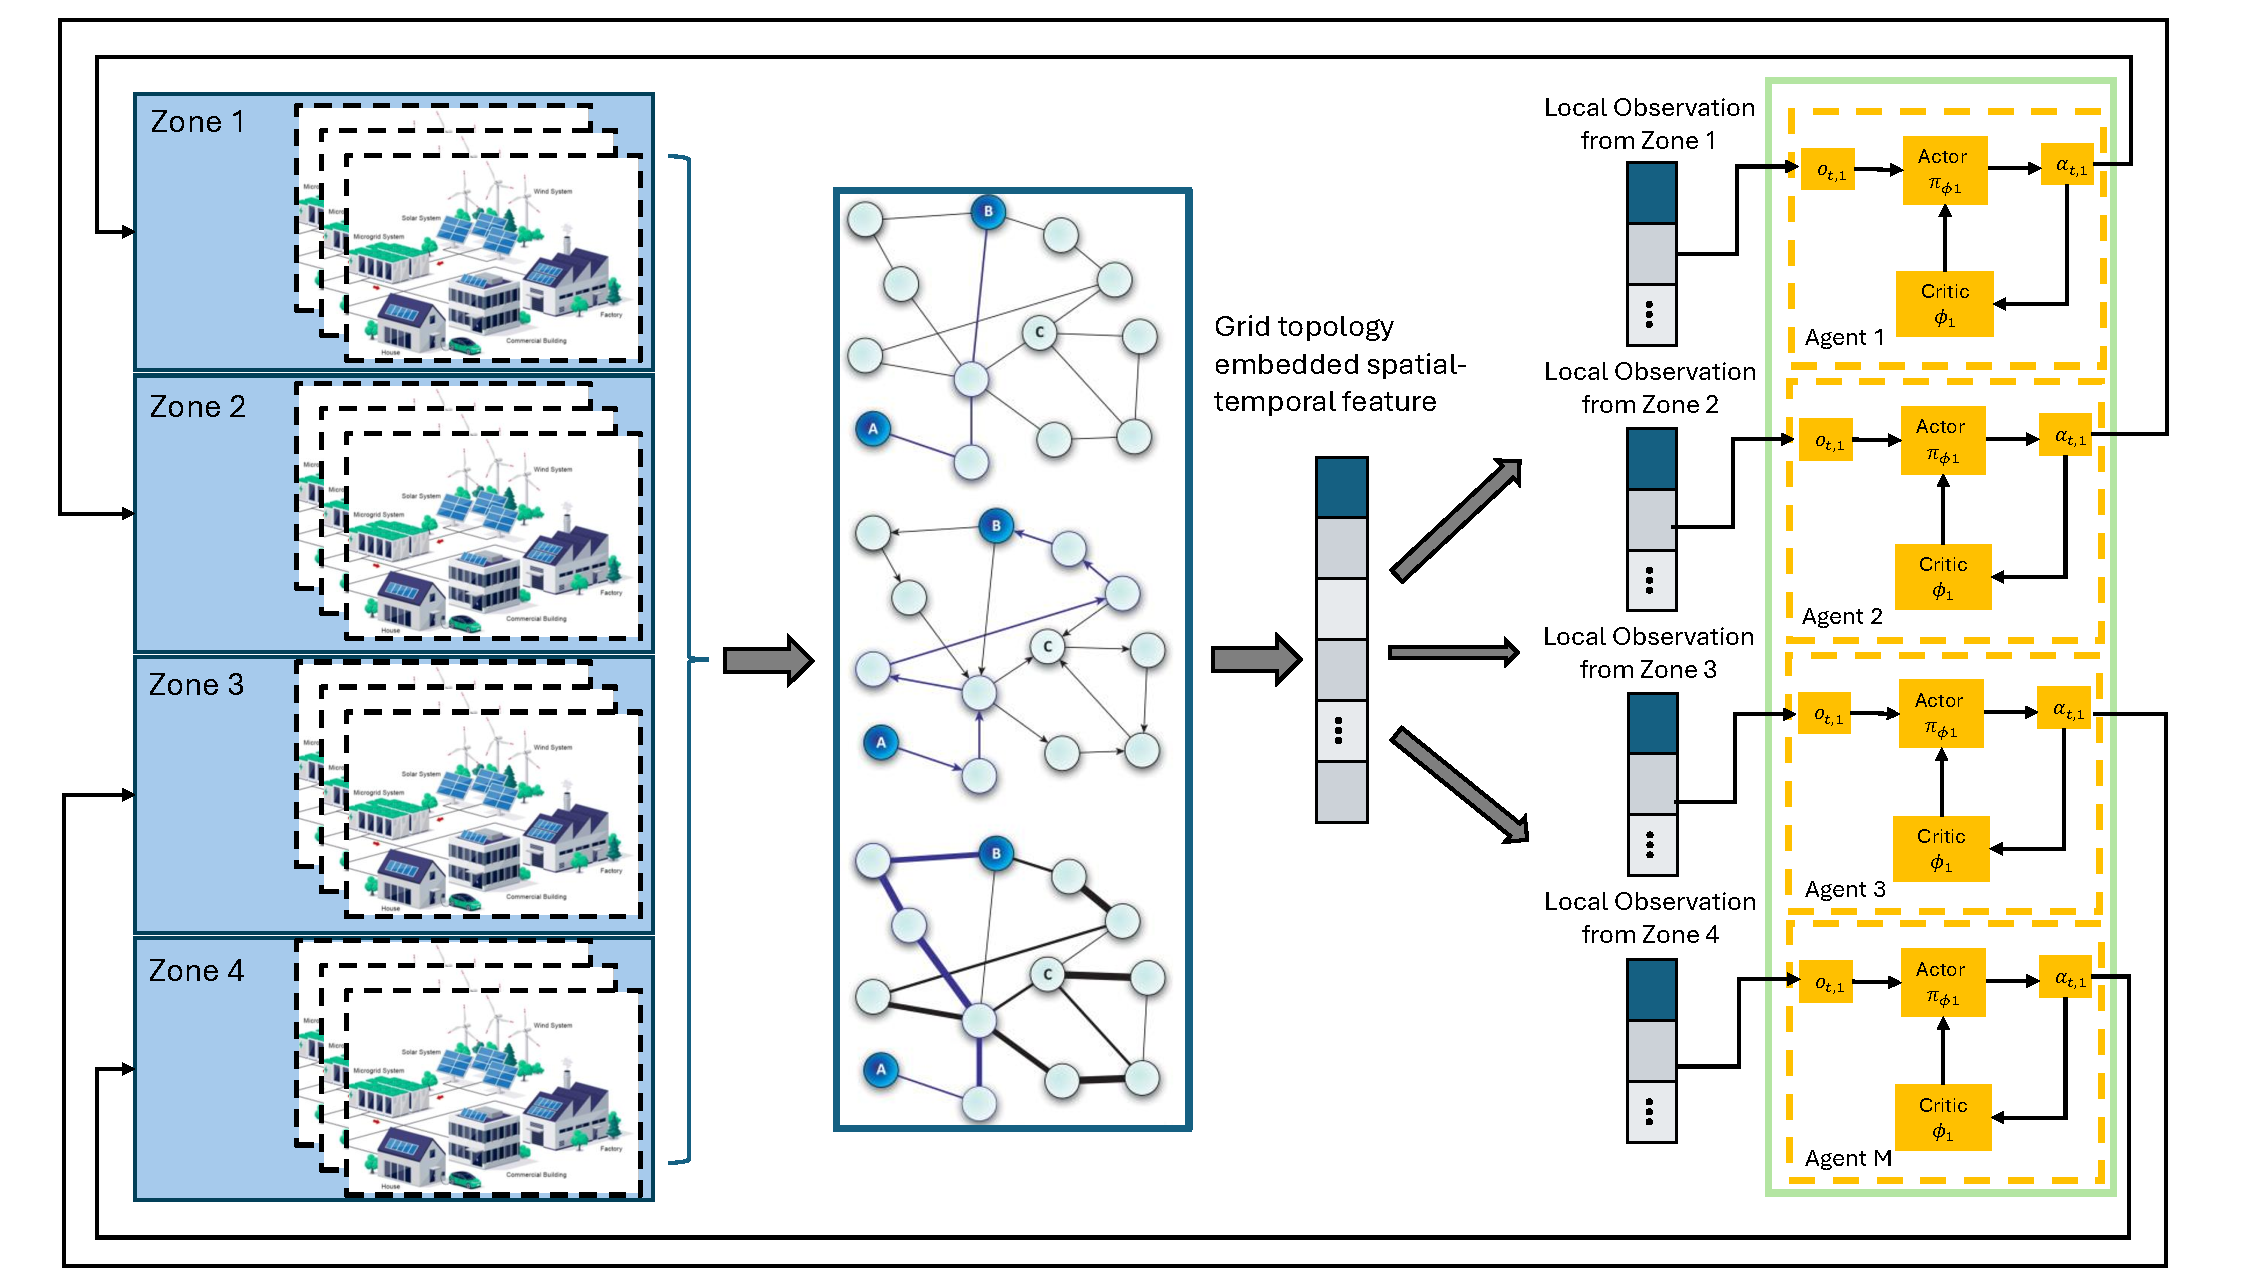
\includegraphics[width=1\linewidth]{img/GraphSAGE-MAPPOargi.pdf}
\caption{Architecture of the proposed GraphSAGE MAPPO controller.}
\label{fig:method_arch}
\end{figure}
% ---------------------------------------------------------------------
\subsection{FFR as a Cooperative Dec-POMDP}
\label{sec:method:mdp}

The overall controller architecture is shown in Fig.~\ref{fig:method_arch}. The 41 GFL agents observe only local and neighborhood information, so the FFR task is a decentralized partially observable Markov decision process (Dec-POMDP) $\langle\mathcal{A},\mathcal{S},\{O_m\},\{U_m\},P,r,\gamma\rangle$ solved under centralized training with decentralized execution (CTDE). The fast step is $\Delta t=1$\,s with 300 steps per episode.

\subsubsection{Observation}
Each agent $m$ observes a 16-dimensional local vector comprising the local frequency deviation and RoCoF read out from \eqref{eq:coi_readout}, net power, SoC and dischargeable-energy headroom, the zonal locational marginal price, a four-way device-type one-hot encoding, VPP membership, the previous droop gain and power reference, SoC violation flags, a persistence power forecast, and a departure proxy. The local vectors are placed on the 123-bus graph at their host buses and augmented with four per-bus grid-background features (active and reactive load, voltage magnitude, and agent density), giving the full feeder observation $\mathit{obs}_{\mathrm{full}}\in\mathbb{R}^{123\times20}$.

\subsubsection{Action}
Each agent emits a two-dimensional action $a_m=[a^P_m,\,a^K_m]\in[-1,1]^2$ that jointly sets a fast active-power reference and a local droop gain, replacing the fixed-gain response $\Delta P^{\mathrm{ffr}}_{i,t}=-K_i\,\Delta f_t$ of the classical loop with a learned, state-conditioned one,
\begin{align}
  \Delta P_m &= a^P_m\cdot 0.1\,P_{\mathrm{rated},m},
  \label{eq:action_power}\\
  K_m &= K_{\min,m}+\tfrac{1}{2}\big(1+a^K_m\big)\big(K_{\max,m}-K_{\min,m}\big).
  \label{eq:action_droop}
\end{align}
The power channel spans up to $\pm10\,\%$ of rated power (clipped to the device rating and SoC headroom, slew-limited at $0.2$/step); the droop channel spans $[K_{\min,m},K_{\max,m}]$ with $K_{\min,m}=0$ and per-type ceilings listed in Table~\ref{tab:system}. A droop gain is enabled only when $\mathrm{SoC}_m$ lies in the FFR-eligibility band, nested inside the physical band (Table~\ref{tab:system}); otherwise $K_m=0$. Exposing $a^P_m$ and $a^K_m$ jointly lets the policy pre-position storage ahead of an anticipated FFR call and trade transient performance against service-quality constraints, which neither a power-only nor a droop-only formulation can do.
\subsubsection{Reward}
A single team reward couples frequency security, control effort, and service quality,

\begin{equation}
  r_t = r^{\Delta f}_t + r^{\mathrm{nadir}}_t + r^{\mathrm{viol}}_t
        + r^{\mathrm{ffr}}_t + r^{\mathrm{eff}}_t + r^{\mathrm{soc}}_t
        + r^{\mathrm{mkt}}_t + r^{\mathrm{commit}}_t,
  \label{eq:reward}
\end{equation}

where the frequency, nadir, and violation terms penalize the COI deviation \eqref{eq:coi_readout} from $f_0$ and its excursions beyond the safe band---the same security target used for evaluation and applied identically to every controller, including the baselines---the FFR-bonus term rewards staying within it, and the effort, SoC, market, and commitment terms regularize the action, penalize SoC violation, credit market revenue, and discourage abrupt gain changes. Error terms are normalized to $[0,1]$ against event-scaled references and combined by fixed weights; the explicit forms and weights are listed in Section~\ref{sec:casestudy}. The RoCoF term is disabled because peak RoCoF is governed by the GFM backbone rather than by the GFL action (Section~\ref{sec:method:safety}). The reward is passed through a running normalizer ($\gamma=0.99$, clipped at $\pm10$).

% ---------------------------------------------------------------------
\subsection{Multi-Agent PPO under CTDE}
\label{sec:method:mappo}

The controller is trained with multi-agent proximal policy optimization (MAPPO) \cite{yu2022mappoeffective,schulman2017ppo} under CTDE: a centralized critic uses global information during training, while each agent executes from ts local observation alone at run time. Both the actor and the critic operate on the per-agent embeddings produced by the encoder of Section~\ref{sec:method:graphsage}.

\emph{Actor.} A single parameter-shared diagonal-Gaussian policy maps each agent embedding through a two-layer perceptron to the mean and log-standard deviation of the two-dimensional action, with a bounded mean $\mu=0.75\tanh(\cdot)$ and $\sigma=\operatorname{softplus}(\cdot)+0.05$. Parameter sharing keeps the policy size independent of $|\mathcal{A}|$ and permits a varying agent count across topologies.

\emph{Critic.} A centralized critic concatenates each agent embedding with a global context formed by mean- and max-pooling over all agents and returns a per-agent value. The per-agent value retains credit information for each DER while the pooled context supplies the system-level signal needed for cooperative coordination.

\emph{Update.} Advantages are estimated by generalized advantage estimation ($\gamma=0.99$, $\lambda=0.95$) from the shared team reward
\eqref{eq:reward}, and the policy is updated by the clipped PPO surrogate 
\begin{equation}
  \mathcal{L}^{\mathrm{clip}}
   = -\,\mathbb{E}\!\left[
       \min\!\big(\rho_t\hat{A}_t,\
       \operatorname{clip}(\rho_t,1-\epsilon,1+\epsilon)\hat{A}_t\big)\right],
  \label{eq:ppo_clip}
\end{equation}
with clip range $\epsilon=0.2$. The total loss adds a value-regression term (coefficient $0.5$) and an entropy bonus annealed across the training curriculum.

% ---------------------------------------------------------------------
\subsection{Inductive GraphSAGE Encoder}
\label{sec:method:graphsage}

The encoder is the component that makes the controller transferable to unseen feeder configurations. We use an inductive GraphSAGE encoder
\cite{hamilton2017graphsage}, which learns aggregator \emph{functions} over node neighborhoods rather than a fixed per-node embedding. For node $j$ at layer $k$,
\begin{equation}
  H_j^{(k)}
   = \sigma\!\Big(W_{\mathrm{self}}\,H_j^{(k-1)}
     + W_{\mathrm{neigh}}\!\cdot\!
       \operatorname{mean}_{u\in\mathcal{N}(j)} H_u^{(k-1)}\Big),
  \label{eq:graphsage}
\end{equation}
where $H_j^{(0)}$ is the per-bus observation and the aggregator weights are shared across all nodes and topologies. We use two layers, mapping the 20-dimensional input to a 128-dimensional hidden layer with ReLU and then to a 128-dimensional embedding.

\emph{Why inductive enables zero-shot transfer.} The edge index of $\mathcal{N}(j)$ in \eqref{eq:graphsage} is rebuilt at every step from the
active feeder graph $\mathcal{G}_t$. Because the learned weights are properties of the aggregator and not of any specific adjacency matrix, the same encoder applies to a topology never seen in training: reconfiguration changes which neighbors are summed in \eqref{eq:graphsage} but not the function that aggregates them. This is the structural difference from transductive graph-convolution encoders, whose spectral filters are tied to a fixed adjacency and must be retrained when the graph changes. The inductive construction is what lets a single controller satisfy the topology-coupled deliverability relation \eqref{eq:deliverability} across configurations without per-topology retraining.

\emph{Embedding extraction.} After two aggregation passes over the 123-bus graph, the embeddings at the 41 DER host buses are extracted and passed to the actor and the centralized critic of Section~\ref{sec:method:mappo}. Both heads therefore reason over a representation that already encodes the neighborhood structure of the realized feeder.

% ---------------------------------------------------------------------
\subsection{Shared Safety Envelope}
\label{sec:method:safety}

Frequency security is enforced by an envelope that is a property of the environment, not of any particular controller; the proposed policy and every baseline of Section~\ref{sec:casestudy} act inside the same envelope. The comparison therefore isolates performance and generalization within the safe set, not safety itself. The envelope rests on four mechanisms.

\emph{Stability by construction.} The map \eqref{eq:action_droop} with $K_{\min}=0$ keeps the droop gains non-negative, so the damping matrix
$D(K_t)=\operatorname{diag}(K_t)\succeq 0$ and the realized droop $-K_m\Delta f_t$ is monotone non-increasing in frequency \cite{feng2022stabilityrl,alduaij2025partialmonotone}.

\emph{Lyapunov certificate.} For the swing energy $V=\tfrac12\Delta\boldsymbol{\omega}^{\!\top}M\Delta\boldsymbol{\omega}+\tfrac12\Delta\boldsymbol{\delta}_{\mathrm{rel}}^{\!\top}\tilde{J}_r\Delta\boldsymbol{\delta}_{\mathrm{rel}}$, the derivative along \eqref{eq:statespace} is $\dot V=-\Delta\boldsymbol{\omega}^{\!\top}D(K_t)\Delta\boldsymbol{\omega}\le0$.
Since $A_f$ in \eqref{eq:af_matrix} is affine in $K_t$ through $D(K_t)$, the vertices of the droop-gain box are extremal and a finite vertex check certifies Hurwitz stability over the full topology-by-gain set; the derivation is given in the Appendix.

\emph{RoCoF by system design.} The peak RoCoF satisfies $\dot f=\Delta P_{\mathrm{imb}}/(2H_{\mathrm{backbone}})$ and is set by the VSG backbone inertia, not by the GFL action in the first step \cite{kenyon2021gfmfreqorder}. The RoCoF reward term is consequently disabled in \eqref{eq:reward}.

\emph{Nadir projection.} A closed-form minimal-perturbation projection of $\Delta P_{\mathrm{ref}}$ keeps the predicted next-step COI deviation within $[-\delta,+\delta]$ ($\delta=0.5$\,Hz), using an affine predictor that mirrors the ZOH dynamics \eqref{eq:zoh}--\eqref{eq:coi_readout} with the located disturbance forcing \eqref{eq:bnet}. A single linear constraint gives a closed form with no quadratic program \cite{tabas2021safefilter}. The guard acts on the COI because that is the resolvable system-frequency observable at the control step and the quantity the controller is rewarded and evaluated on. The projection is a model-level guarantee under the assumptions of Section~\ref{sec:model:freqmodel}; an EMT/hardware-in-the-loop certificate is left to future work.

% =====================================================================
\section{Case Study}
\label{sec:casestudy}


% NOTE: numeric values flagged [TBD] are pending regeneration on the
% unified VSG model; all other values are taken from the verified spec.

% ---------------------------------------------------------------------
\subsection{Test System}
\label{sec:casestudy:system}

The controller is evaluated on a modified IEEE 123-bus distribution feeder operated as a 100\,\% inverter-based islanded microgrid  Fig.~\ref{fig:topology}). System and device parameters are summarized in Table~\ref{tab:system}; the frequency-security thresholds, taken from the ENTSO-E network codes and IEEE standards, are summarized in Table~\ref{tab:fsec_standards}.


\begin{figure}[!t]
\centering
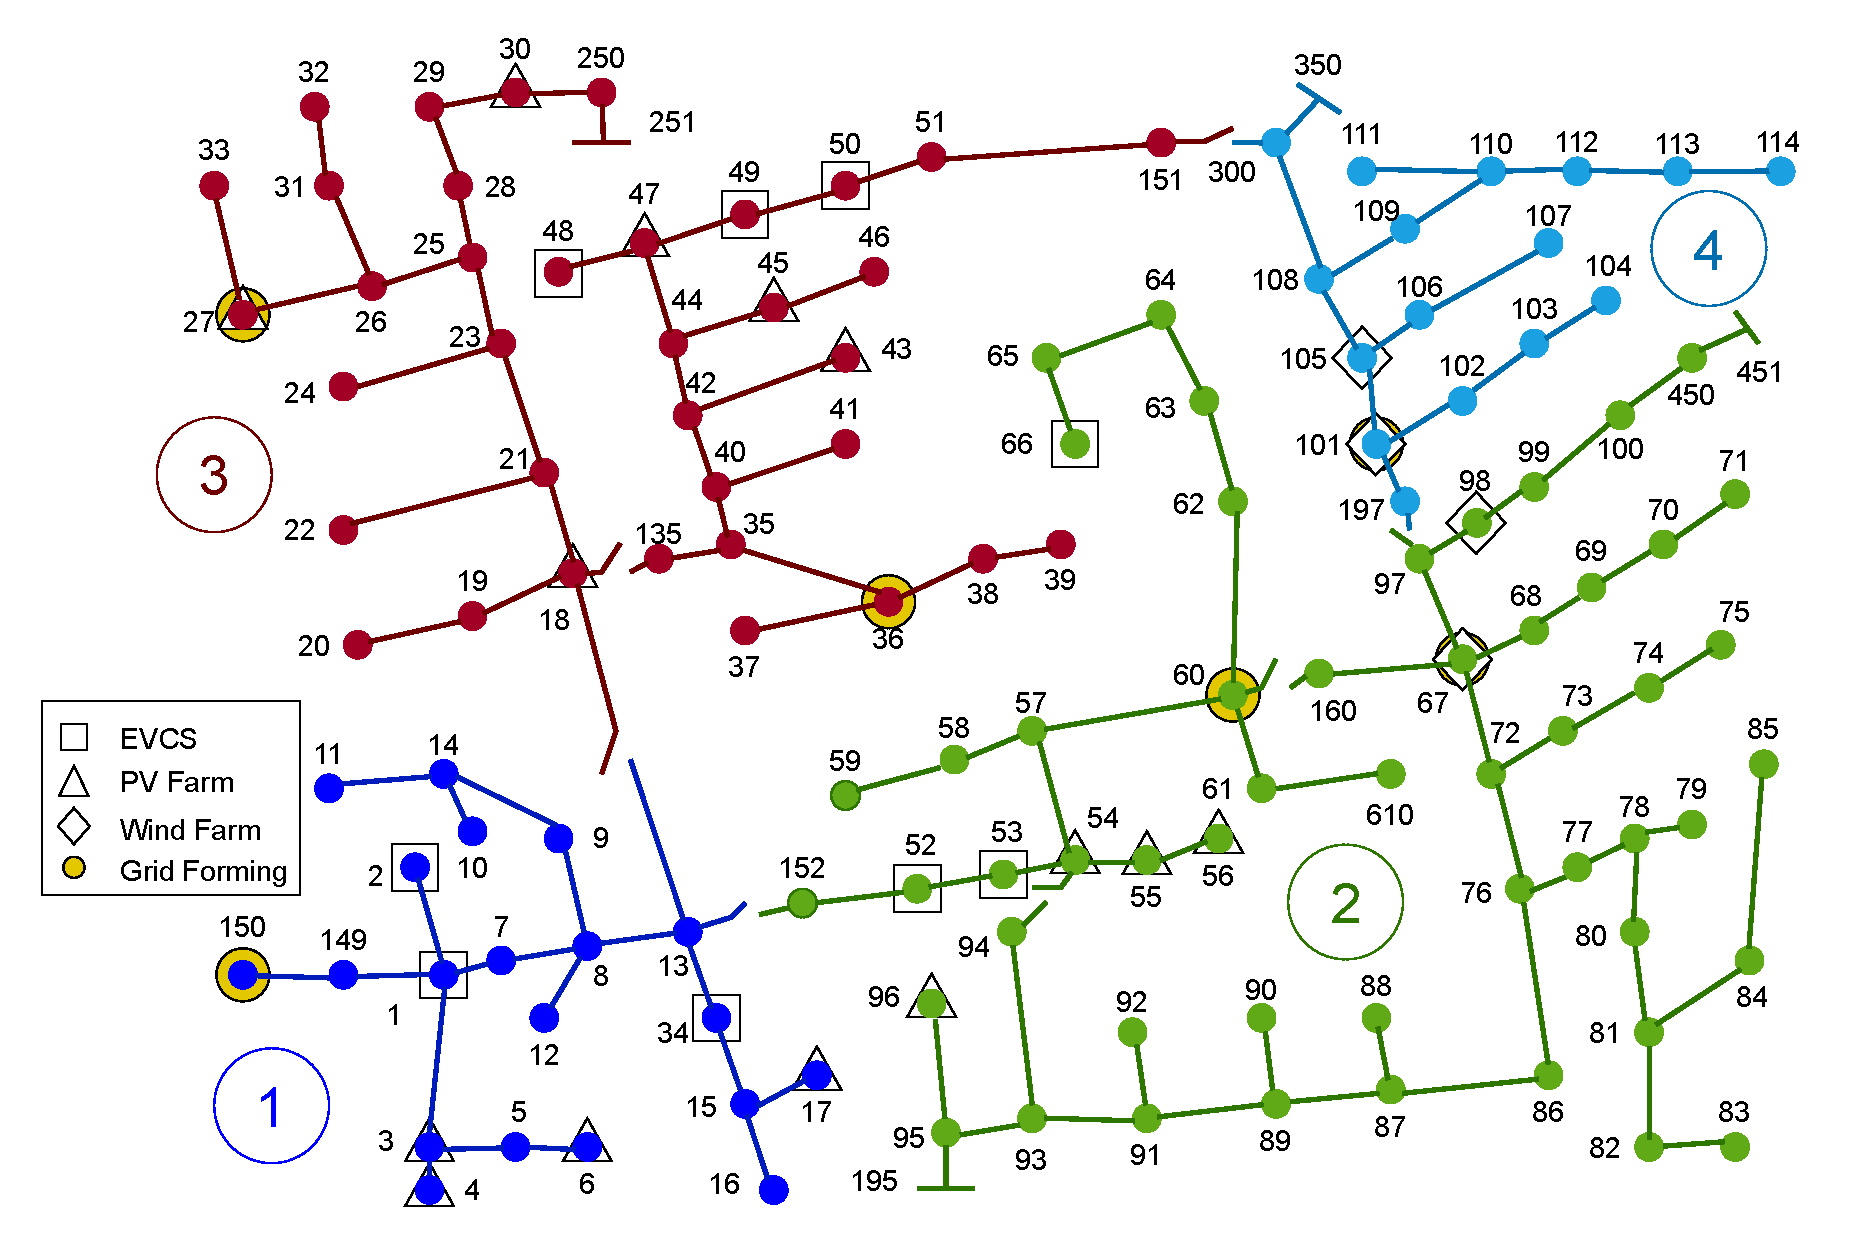
\includegraphics[width=0.95\linewidth]{img/Topology.pdf}
\caption{Topology of the islanded IEEE 123-bus feeder after VPP-zone partitioning.}
\label{fig:topology}
\end{figure}


\begin{table}[!h]
\caption{Test-System and Device Parameters}
\label{tab:system}
\centering
\footnotesize
\resizebox{\linewidth}{!}{
\begin{tabular}{lll}
\toprule
Quantity & Symbol & Value \\
\midrule
Base power, frequency & $S_{\mathrm{base}}, f_0$ & $15.7$\,MW, $50$\,Hz \\
GFM backbone (VSG / droop) & $n_g, H_g$ & $6$ ($2.0$\,s / $0.5$\,s) \\
Aggregate system inertia & $H_{\mathrm{sys}}$ & $1.34$\,s \\
GFL agents, VPP zones & $|\mathcal{A}|, |\mathcal{Z}|$ & 41 agents, 34 zones \\
Droop ceiling (BESS/V2G/DPV) & $K_{\max}$ & $0.30$ / $0.20$ / $0.15 \cdot P_{\mathrm{rated}}$ \\
SoC band (Physical / FFR) & --- & $[0.20, 0.90]$ / $[0.25, 0.85]$ \\
Efficiency, V2G response lag & $\eta, T_{\mathrm{v2g}}$ & $0.95$, $0.3$\,s \\
Time step, Episode length & $\Delta t$ & $1$\,s / $300$ steps \\
\bottomrule
\end{tabular}
}
\end{table}

\begin{table}[!t]
\caption{Frequency-security thresholds and the cited standard
defining each value.}
\label{tab:fsec_standards}
\centering
\footnotesize
\resizebox{\linewidth}{!}{
\begin{tabular}{lll}
\toprule
Quantity & Value & Source \\
\midrule
UFLS Stage 1 trip       & $49.0$~Hz       & ENTSO-E SO~GL Art.~11~\cite{entsoe_sogl_2017} \\
Operator alarm / FFR target & $49.5$~Hz   & FFR margin $\Delta f^{\max}=0.5$~Hz                \\
UFLS Stage 1 delay      & $300$~ms        & IEEE Std C37.117-2007~\cite{ieee_c37117_2007}      \\
RoCoF ride-through      & $2.0$~Hz/s      & IEEE Std 1547-2018 Cat.~III~\cite{ieee_1547_2018}  \\
FCR full activation     & $\pm 200$~mHz   & ENTSO-E SO~GL Art.~14~\cite{entsoe_sogl_2017}      \\
Voltage THD limit (MV)  & $5$\,\%         & IEEE Std 519-2014~\cite{ieee_519_2014}             \\
\bottomrule
\end{tabular}
}
\end{table}
% ---------------------------------------------------------------------
\subsection{Disturbance Scenarios and Topology Hold-Out}
\label{sec:casestudy:scenarios}

The controller is exercised with four disturbance classes load step, generation trip, line trip, and high-renewable surge scaled as a fraction of $S_{\mathrm{base}}$ (Table~\ref{tab:scenarios}). Topology generalization is assessed under a zero-shot hold-out protocol: the set of feeder configurations is partitioned by farthest-point sampling on the Jaccard edge distance into disjoint training and testing sets,
\begin{equation}
  \mathcal{G}_{\mathrm{train}}\cap\mathcal{G}_{\mathrm{test}}=\varnothing,
  \label{eq:holdout}
\end{equation}
so that every test topology---generated by tie-switch reconfiguration or an $N{-}1$ line contingency is unseen during training. Held-out configurations differ from the nearest training topology by a Jaccard edge distance of up to $\approx\!0.18$, an order of magnitude above a naive random-reconfiguration split. We note that reconfiguration of a radial feeder changes only a bounded fraction of edges, so this protocol stresses structural generalization within the reachable configuration space rather than transfer to arbitrary graphs; within that space the hold-out is demanding.

\begin{table}[!t]
\caption{Contingency scenarios.}
\label{tab:scenarios}
\centering
\footnotesize
\resizebox{\linewidth}{!}{
\begin{tabular}{llccc}
\toprule
Sc. & Event       & $\Delta P$ (MW) & \% $S_{\mathrm{base}}$ & Purpose \\
\midrule
S1  & load step             & +2.5 & 16 & moderate          \\
S2  & generation trip       & -3.9 & 25 & severe under-freq. \\
S3  & line trip             &  2.4 & 15 & topology mutation  \\
S4  & high-renewable surge  & +4.7 & 30 & over-freq. stress  \\
\bottomrule
\end{tabular}
}
\end{table}

% ---------------------------------------------------------------------
\subsection{Baselines}
\label{sec:casestudy:baselines}

The proposed controller is compared against five baselines spanning non-learning references, a state-of-the-art multi-agent method, a transductive graph encoder, and an encoder ablation (Table~\ref{tab:baselines}). All learning baselines run in the identical environment, observation, dual action, reward, and shared safety envelope of Sections~\ref{sec:model} \ref{sec:method}; only the encoder or learning algorithm differs. The comparison therefore isolates the contribution of each architectural component within a common safe operating envelope, rather than safety itself. In particular, the MLP-MAPPO row isolates the value of graph message-passing, since its only difference from the proposed controller is the encoder. GCNN-PPO is a transductive spectral-GCN reference; because it is single-centralized it differs from the proposed controller in \emph{both} the encoder and the agent structure, so it serves as a realistic state-of-the-art comparator rather than a clean inductive-versus-transductive control. The inductive property itself is evidenced directly by the near-flat IAE-versus-edge-distance profile of Fig.~\ref{fig:fig6}, not by this row.


\begin{table}[!h]
\caption{Baselines and Isolated Component}
\label{tab:methods}
\centering
\footnotesize
\resizebox{\linewidth}{!}{
\begin{tabular}{lllll}
\toprule
\# & Method & Encoder & RL algorithm & Multi-agent \\
\midrule
1 & GraphSAGE-MAPPO (\emph{ours}) & GraphSAGE   & PPO  & MAPPO (CTDE)         \\
2 & MLP-MAPPO (ablation)          & MLP         & PPO  & MAPPO (CTDE)         \\
3 & GCNN-PPO~\cite{guo2024gcnnppo}& Spectral GCN& PPO  & Single centralized   \\
4 & MATD3~\cite{li2025matd3}      & MLP         & TD3  & CTDE                 \\
5 & Fixed droop                   & ---         & ---  & ---                  \\
6 & No FFR                        & ---         & ---  & ---                  \\
\bottomrule
\end{tabular}
}
\end{table}
% ---------------------------------------------------------------------
\subsection{Training Protocol and Hyperparameters}
\label{sec:casestudy:training}

Training uses a six-phase disturbance curriculum that progressively increases event magnitude and probability, under centralized training with decentralized execution. This curriculum is a fixed training schedule; it is distinct from the hyperparameter search described next. The hyperparameters of the proposed controller are selected by asynchronous successive halving (ASHA) screening on a composite frequency-security score, yielding the values in Table~\ref{tab:hyperparams}. To keep the comparison fair, every learning baseline runs in the identical environment, observation, dual action, reward, curriculum, optimizer, and training step budget, and is given the \emph{same tuned capacity}---embedding/hidden width, number of layers, and PPO settings---as the proposed controller, so the proposed method enjoys no capacity or schedule advantage; only the encoder (or, for GCNN-PPO, the encoder and the centralized agent structure) differs. The training curves of the proposed controller and the learning baselines are shown in Fig.~\ref{fig:learning_curve}, which confirms that each method is reported at its converged performance.

\begin{table}[t]
  \centering
  \caption{Selected hyperparameters (ASHA-tuned on the proposed controller; the same capacity is shared by all learning baselines).}
  \label{tab:hyperparams}
  \begin{tabular}{lll}
    \hline
    Hyperparameter & Symbol & Value\\
    \hline
    Learning rate          & ---            & [TBD]\\
    Discount / GAE         & $\gamma,\lambda$ & $0.99$, $0.95$\\
    PPO clip               & $\epsilon$     & $0.2$\\
    Entropy coefficient    & ---            & [TBD]\\
    Embedding / hidden dim & ---            & $128$\,/\,$128$\\
    GraphSAGE layers       & ---            & $2$\\
    Update epochs / minibatch & ---         & [TBD]\\
    Curriculum length      & ---            & [TBD] episodes\\
    \hline
  \end{tabular}
\end{table}

\begin{figure}[t]
  \centering
  % \includegraphics[width=\columnwidth]{fig/learning_curve.pdf}
  \caption{Training curves (episodic return vs.\ episode) for the proposed controller and the learning baselines under the six-phase curriculum. Shaded bands denote $\pm1\sigma$ over training seeds. [Figure pending regeneration on the unified VSG model.]}
  \label{fig:learning_curve}
\end{figure}

% ---------------------------------------------------------------------
\subsection{Evaluation Metrics and Statistical Protocol}
\label{sec:casestudy:metrics}

Performance is reported across four metric groups: (i) frequency security nadir, maximum RoCoF, IAE, settling time, and FFR success rate against the UFLS thresholds; (ii) service and economics committed reserve and energy plus capacity revenue; (iii) power quality voltage THD at the point of common coupling; and (iv) topology generalization the hold-out IAE gap and the slope of IAE versus Jaccard edge distance from the training set. The held-out topology set is the primary experimental factor: each learning controller is evaluated on the same disjoint set of unseen feeder configurations, and each per-topology value is itself averaged over repeated episodes with randomized operating points and event timing. Unless stated otherwise, table entries report the mean across the held-out topologies with a $95\,\%$ confidence interval, and the difference between the proposed controller and the next-best method on IAE and nadir is assessed by a paired Wilcoxon signed-rank test over the matched per-topology values. Because reinforcement-learning outcomes can be seed-sensitive, the proposed controller is additionally trained from three independent random seeds; the topology-generalization result is reported as the mean across seeds and is consistent across all three.



\section{Results and Discussion}
\label{sec:results}
 
Fig.~\ref{fig:radar_overview} summarizes the evaluation: for each of the four contingencies, the six controllers are scored on five axes spanning the technical and economic objectives post-event IAE, nadir margin, settling speed, topology robustness, and DSO cost efficiency. Each axis is oriented so that larger is better, grounded at zero, and normalized by the best in-group value, so the enclosed areas are directly comparable. The proposed controller encloses the largest area in S1-S3 and remains competitive on the over-frequency surge~S4, and it is the only method strong on the technical and the economic axes at once. The following subsections quantify each axis and isolate the mechanism; they do not restate the overview.
 
\begin{figure*}[!t]
\centering
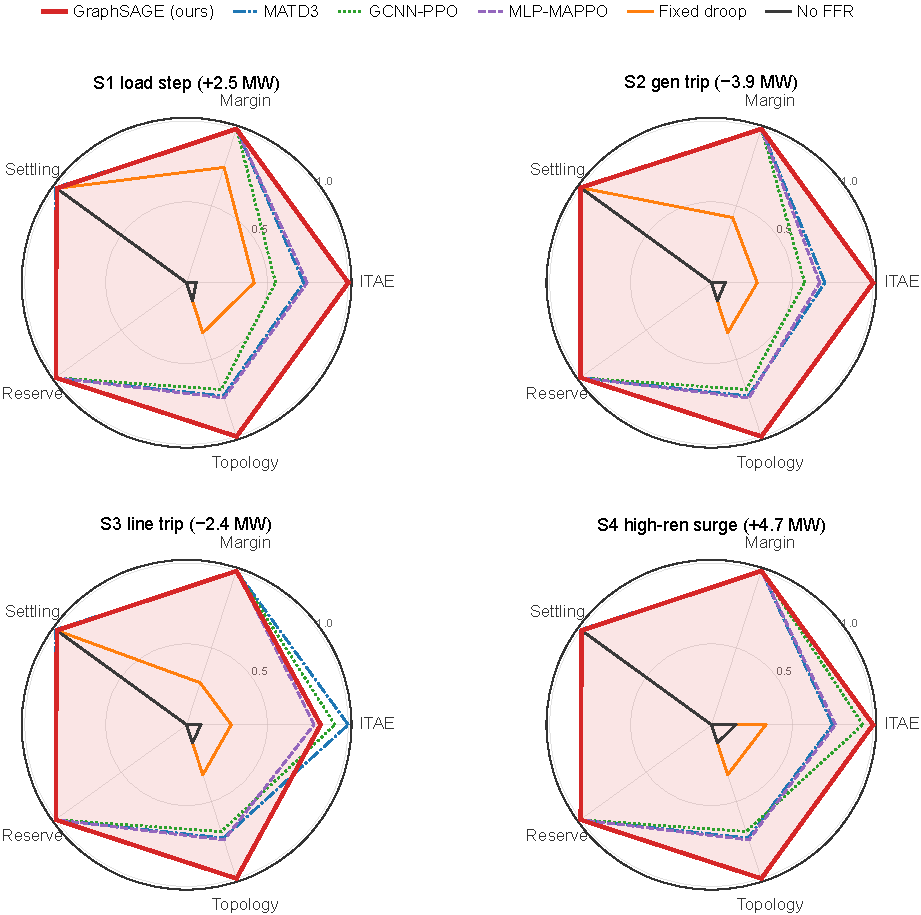
\includegraphics[width=0.98\textwidth]{img/fig1_radar.pdf}
\caption{Per-scenario performance radar for the four contingencies (origin at zero, each axis normalized by the best in-group value within the panel). The topology robustness and DSO cost efficiency axes are system-level and therefore identical across panels.}
\label{fig:radar_overview}
\end{figure*}
 
% ==================================================================
\subsection{Frequency-Security Performance}
\label{ssec:res_stability}
% ==================================================================
 
Table~\ref{tab:ffr_main} reports the per-scenario frequency-security metrics, each entry being the mean over $20$ evaluation episodes per training topology with randomized operating point and event timing ($20\times 11=220$ rollouts), reported with its standard deviation; the per-topology breakdown and the across-topology dispersion on the unseen split are given in Table~\ref{tab:topo} and the paired-significance analysis of Section~\ref{ssec:res_topo}. Fig.~\ref{fig:freq_grid} overlays the corresponding mean frequency trajectories ($\pm 1\sigma$ band) for the six controllers.
 
\begin{table*}[!t]
\caption{Frequency-security performance per scenario (mean $\pm$ SD over $20$ evaluation episodes per topology across the $11$ training topologies; $220$ rollouts).}
\label{tab:ffr_main}
\centering
\footnotesize
\begin{tabular}{llccccc}
\toprule
Scenario & Method & Nadir/Zenith (Hz) & RoCoF$_{\max}$ (Hz/s) &
IAE$_{\mathrm{post}}$ (Hz$\cdot$s) & ITAE (Hz$\cdot$s$^{2}$) &
$t_{\mathrm{settle}}$ (s) \\
\midrule
\multirow{6}{*}{S1 -- load step}
  & GraphSAGE-MAPPO (\emph{ours}) & \textbf{49.71} & 3.05          & \textbf{0.82}  & \textbf{444.3}  & \textbf{7.3}  \\
  & MLP-MAPPO (ablation)          & 49.41          & 3.97          & 11.18          & 8301.7          & 49.9          \\
  & GCNN-PPO                      & 49.65          & 2.87          & 5.78           & 5039.0          & 50.0          \\
  & MATD3                         & 49.66          & 2.60          & 1.70           & 950.4           & 23.2          \\
  & Fixed droop                   & 49.34          & 2.19          & 3.31           & 453.2           & 16.2          \\
  & No FFR                        & 49.37          & \textbf{1.65} & 3.61           & 506.7           & 15.4          \\
\midrule
\multirow{6}{*}{S2 -- gen trip}
  & GraphSAGE-MAPPO (\emph{ours}) & \textbf{49.71} & \textbf{2.35} & \textbf{1.22}  & \textbf{227.1}  & \textbf{7.8}  \\
  & MLP-MAPPO (ablation)          & 49.37          & 4.15          & 10.35          & 7473.5          & 47.5          \\
  & GCNN-PPO                      & 49.63          & 3.41          & 5.06           & 3532.4          & 49.6          \\
  & MATD3                         & 49.61          & \textbf{2.35} & 3.71           & 1858.1          & 49.2          \\
  & Fixed droop                   & 48.97          & 3.21          & 4.78           & 393.5           & 16.0          \\
  & No FFR                        & 49.02          & 2.56          & 5.57           & 523.9           & 17.2          \\
\midrule
\multirow{6}{*}{S3 -- line trip}
  & GraphSAGE-MAPPO (\emph{ours}) & \textbf{49.71} & 3.05          & \textbf{0.82}  & 457.3           & \textbf{6.8}  \\
  & MLP-MAPPO (ablation)          & 49.34          & 3.99          & 11.12          & 8841.5          & 48.6          \\
  & GCNN-PPO                      & 49.62          & 3.07          & 6.06           & 5458.6          & 49.8          \\
  & MATD3                         & 49.66          & 2.34          & 2.40           & 1391.1          & 25.2          \\
  & Fixed droop                   & 49.36          & 2.10          & 3.19           & \textbf{388.6}  & 16.9          \\
  & No FFR                        & 49.40          & \textbf{1.58} & 3.48           & 505.0           & 15.3          \\
\midrule
\multirow{6}{*}{S4 -- high-ren. surge}
  & GraphSAGE-MAPPO (\emph{ours}) & \textbf{50.01} & \textbf{3.00} & 4.09           & 2230.1          & 22.8          \\
  & MLP-MAPPO (ablation)          & 50.59          & 3.63          & 11.87          & 9303.3          & 50.0          \\
  & GCNN-PPO                      & 50.51          & 3.78          & 5.89           & 3891.1          & 49.9          \\
  & MATD3                         & 50.31          & 3.73          & \textbf{3.42}  & \textbf{1381.2} & 22.5          \\
  & Fixed droop                   & 51.26          & 3.45          & 9.82           & 4320.1          & 45.1          \\
  & No FFR                        & 51.18          & 3.09          & 7.07           & 920.2           & \textbf{19.9} \\
\bottomrule
\end{tabular}
\end{table*}
 
\begin{figure*}[!h]
\centering
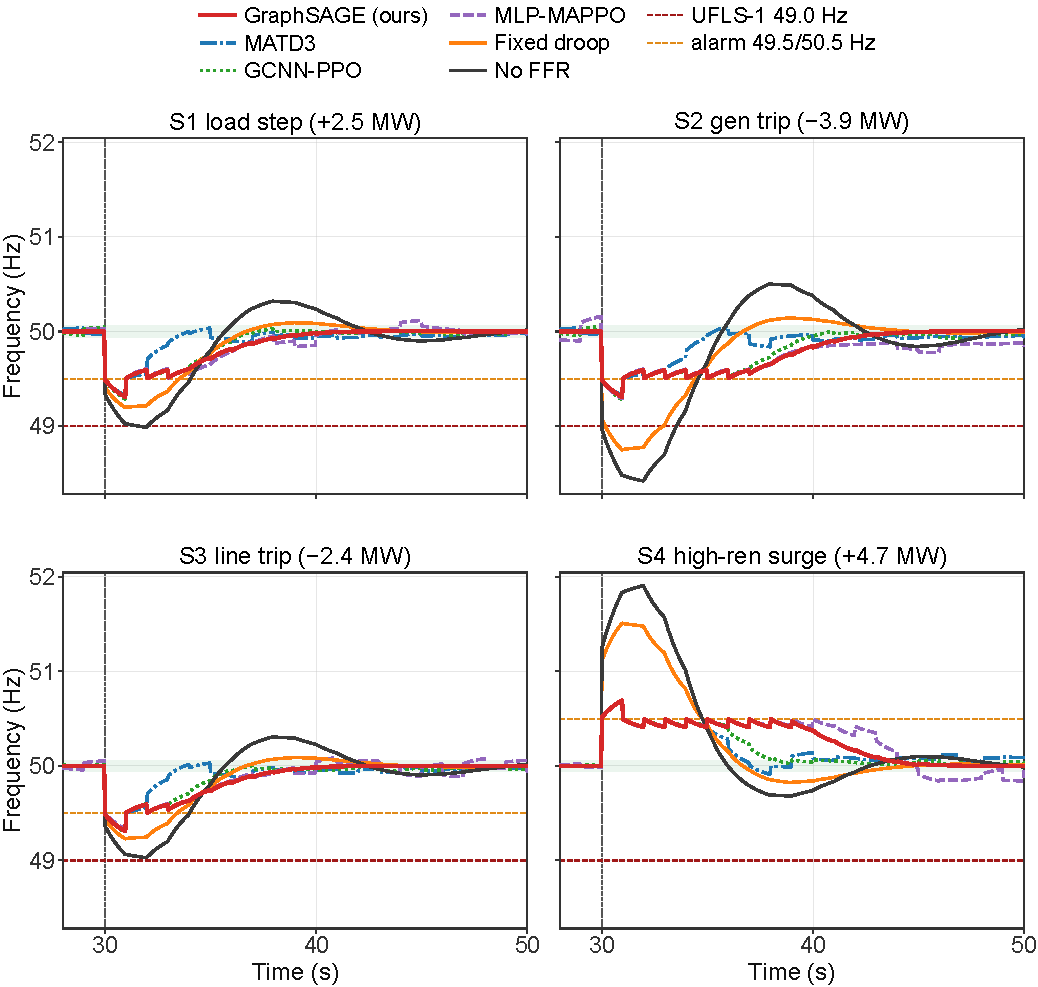
\includegraphics[width=0.95\textwidth]{img/fig_freq_grid.pdf}
\caption{Frequency response (mean $\pm 1\sigma$ over the evaluation episodes), six controllers. Dashed red: UFLS Stage~1 ($49.0$~Hz); dashed orange: $49.5$~Hz alarm; green band: $\pm 0.1$~Hz settling envelope.}
\label{fig:freq_grid}
\end{figure*}
 
\emph{Frequency excursion.}
The proposed controller attains the best post-event nadir (S1-S3) and the lowest over-frequency zenith (S4) in every scenario. On the severe generation trip~S2 it holds the nadir at $49.71$~Hz, a margin of 0.74 Hz over the fixed-droop baseline (48.97 Hz) and the only controller to keep the nadir clear of the 49.5 Hz alarm. On the over-frequency surge~S4 it limits the peak to 50.01 Hz against 51.26 Hz for fixed droop, reducing the over-frequency excursion above nominal from 1.26 Hz to 0.01 Hz.
 
\emph{Integral error and settling.}
The proposed controller reduces IAE$_{\mathrm{post}}$ relative to fixed droop by 75 \% (S1), $74$\,\% (S2), $74$\,\% (S3), and $58$\,\% (S4), and re-enters the $\pm0.1$~Hz band in 6.8-7.8 on S1-S3, 2.0-2.5 times faster than fixed droop (16.0-16.9 s) and $2.0$--$2.3\times$ faster than no FFR. The MLP-MAPPO ablation, which shares the identical RL stack but lacks the inductive graph encoder, fails to settle within the 50 s window and incurs the largest IAE in every scenario, isolating the encoder as the source of the gain (quantified directly in Section~\ref{ssec:res_topo}).
 
\emph{Choice of metrics.}
A frequency-security success rate against the operator alarm band is not reported: that quantity is gated by the maximum RoCoF, which in a 100\,\% inverter-based system is set by the backbone inertia \eqref{eq:hsys} rather than by the grid-following FFR action, and therefore does not discriminate controller performance. The nadir, IAE, and settling time are the operative frequency-security metrics throughout, and the proposed controller leads on all three.
 
\begin{table}[!t]
\caption{Severity scaling on the generation-trip family
($5$ seeds per cell).}
\label{tab:severity}
\centering
\footnotesize
\resizebox{\linewidth}{!}{
\begin{tabular}{lcccccc}
\toprule
$|\Delta P|$ (MW) & No FFR & Droop & MLP & GCNN & MATD3 & \textbf{Ours} \\
\midrule
\multicolumn{7}{c}{\emph{Post-event nadir} (Hz)} \\
\midrule
Mild (2.0)     & 49.31 & 49.27 & 48.96 & 49.53 & 49.59 & \textbf{49.64} \\
Moderate (4.0) & 48.63 & 48.55 & 49.19 & 49.44 & 49.42 & \textbf{49.60} \\
Severe (6.0)   & 48.38 & 48.29 & 48.95 & 49.36 & 49.20 & \textbf{49.38} \\
\midrule
\multicolumn{7}{c}{\emph{Settling time} (s)} \\
\midrule
Mild (2.0)     & 14.6 & 28.7 & 50.0 & 49.8 & 45.8 & \textbf{6.9}  \\
Moderate (4.0) & 18.0 & 15.0 & 50.0 & 49.9 & 49.4 & \textbf{10.0} \\
Severe (6.0)   & 17.0 & 17.6 & 50.0 & 49.9 & 50.0 & 50.0          \\
\bottomrule
\end{tabular}
}
\end{table}
 
\emph{Severity scaling.}
Table~\ref{tab:severity} sweeps the disturbance from $2$ to $6$~MW ($13$--$38$\,\% of $S_{\mathrm{base}}$); the nadir and settling time discriminate the controllers. The proposed controller preserves the highest nadir at every severity level, with the advantage over fixed droop widening from $0.37$~Hz (mild) to $1.09$~Hz (severe). Its settling time is $2$--$4\times$ shorter than every baseline at the mild and moderate levels; at the $6$~MW level all controllers saturate the $50$~s window, so the nadir margin remains the discriminator. The degradation is therefore graceful and monotonic rather than a cliff-style failure.
 
% ==================================================================
\subsection{Topology Generalization}
\label{ssec:res_topo}
% ==================================================================
 
Topology generalization is the central claim and is evaluated in three complementary ways: (i)~the train-to-unseen gap on the $11/5$ disjoint topology split (Table~\ref{tab:topo}); (ii)~a direct encoder-only ablation under the identical RL stack (Table~\ref{tab:encoder}); and (iii)~the slope of IAE$_{\mathrm{post}}$ against Jaccard edge distance (Fig.~\ref{fig:fig6}).
 
\begin{table}[!t]
\caption{Topology generalization on the generation-trip scenario: train ($11$) versus unseen ($5$) topologies.}
\label{tab:topo}
\centering
\footnotesize
\resizebox{\linewidth}{!}{
\begin{tabular}{lccccc}
\toprule
Method & Nadir$_{\mathrm{tr}}$ & Nadir$_{\mathrm{un}}$ &
$\Delta$ (Hz) & IAE$_{\mathrm{tr}}$/IAE$_{\mathrm{un}}$ & Gap (\%) \\
\midrule
GraphSAGE-MAPPO (\emph{ours}) & \textbf{49.71} & \textbf{49.65} & \textbf{$-$0.06} & \textbf{1.22/1.41} & $+16$ \\
MATD3                         & 49.61          & 49.50          & $-$0.11          & 3.80/4.41          & $+16$ \\
GCNN-PPO                      & 49.64          & 49.58          & $-$0.06          & 5.34/6.54          & $+22$ \\
MLP-MAPPO (ablation)          & 49.38          & 49.22          & $-$0.16          & 9.60/13.94         & $+45$ \\
Fixed droop                   & 48.96          & 48.66          & $-$0.30          & 4.81/5.33          & $+11$ \\
No FFR                        & 49.02          & 48.73          & $-$0.29          & 5.60/6.62          & $+18$ \\
\bottomrule
\end{tabular}
}
\end{table}
 
\begin{table}[!t]
\caption{Encoder-only ablation: GraphSAGE versus MLP under an identical RL stack, mean over the four scenarios.}
\label{tab:encoder}
\centering
\footnotesize
\begin{tabular}{lccc}
\toprule
Encoder & IAE$_{\mathrm{post}}$ & Nadir (Hz) & RoCoF$_{\max}$ (Hz/s) \\
\midrule
\textbf{GraphSAGE} & \textbf{1.74}  & \textbf{49.58} & \textbf{2.86} \\
MLP                & 11.13          & 49.33          & 3.93          \\
\bottomrule
\end{tabular}
\end{table}
 
\emph{Train-to-unseen gap.}
In Table~\ref{tab:topo}, $\Delta$ is the unseen-minus-train nadir shift and the gap is the relative increase in IAE$_{\mathrm{post}}$ from the train to the unseen split. On the unseen topologies the proposed controller loses only $0.06$~Hz of nadir margin and holds the best nadir on both splits ($49.71\rightarrow49.65$~Hz). Its IAE$_{\mathrm{post}}$ on the unseen split ($1.41$~Hz$\cdot$s) remains $3.1\times$ lower than the next-best controller (MATD3, $4.41$). The MLP-MAPPO ablation is the most brittle, with IAE growing $45$\,\% across the split versus the proposed controller's $16$\,\%, despite using the same RL stack.
 
\emph{Encoder ablation.}
Table~\ref{tab:encoder} swaps GraphSAGE for an MLP under an otherwise identical stack, isolating the value of graph message-passing. The graph encoder yields a $6.4\times$ lower IAE$_{\mathrm{post}}$ ($1.74$ versus $11.13$~Hz$\cdot$s), a $0.25$~Hz higher nadir, and a $27$\,\% lower maximum RoCoF. This establishes that graph message-passing, not the RL algorithm, drives the gain; that the benefit is specifically the \emph{inductive} re-aggregation over the active edge set rather than a fixed-graph encoding is shown next by the near-flat train-to-unseen profile of Fig.~\ref{fig:fig6}.
 
\begin{figure}[!h]
\centering

\includegraphics[width=0.98\columnwidth]{img/fig_iae_vs_distance.pdf}
\caption{Post-event IAE on the training versus the unseen topologies for each controller; the proposed controller holds the lowest IAE on both splits with the smallest train-to-unseen increase.}
\label{fig:fig6}
\end{figure}
 
\emph{Train-to-unseen transfer.}
Fig.~\ref{fig:fig6} compares IAE$_{\mathrm{post}}$ on the training and the unseen topologies for each controller. The proposed controller holds the lowest IAE on both splits ($1.22\rightarrow1.41$~Hz$\cdot$s) and the smallest train-to-unseen increase, whereas the MLP ablation rises from $9.60$ to $13.94$~Hz$\cdot$s. This is the signature of an inductive encoder that reaggregates over the active edge set in the same forward pass, in contrast to encoders tied to a fixed adjacency.
 
% ==================================================================
\subsection{Economic Efficiency}
\label{ssec:res_econ}
% ==================================================================
 
This subsection evaluates the controller as a \emph{price taker} against the DLMP and reserve prices cleared/bid in the upper layers (Section~\ref{sec:model:layers}): the prices are inputs to Layer 2, and the comparison reports the DSO settlement that each controller induces under the common price deck \cite{rahimiyan2016pricetaker,li2014dlmp}. Table~\ref{tab:econ} reports the DSO procurement cost under the configured price deck (ENTSO-E-aligned capacity and activation tariffs, Nordic-style undersupply multiplier $c_{\mathrm{us}}=3$), the committed reserve per event, and the reserve-delivery success rate. Costs are reported per event and per \emph{secured} event (the per-event DSO payment normalized by the reserve-delivery success rate); the undersupply column is the shortfall-penalty exposure, for which lower is better.
 
\begin{table*}[!t]
\caption{Economic comparison on the generation-trip scenario
($5$ seeds per cell).}
\label{tab:econ}
\centering
\footnotesize
\begin{tabular}{lccccc}
\toprule
Method & Delivery SR & Committed (MW/ev.) & EUR/event & EUR/secured ev. & Undersupply (EUR/ev.) \\
\midrule
GraphSAGE-MAPPO (\emph{ours}) & \textbf{1.00} & \textbf{0.086} & \textbf{0.356} & \textbf{0.357} & \textbf{0.00} \\
MLP-MAPPO                     & 1.00          & 0.228          & 0.951          & 0.952          & 9.78  \\
GCNN-PPO                      & 0.95          & 0.225          & 0.939          & 0.989          & 16.07 \\
MATD3                         & 1.00          & 0.265          & 1.104          & 1.105          & 5.01  \\
Fixed droop                   & 0.25          & ---            & 0.029          & 0.114          & 0.56  \\
No FFR                        & 0.25          & ---            & 0.005          & 0.021          & 0.00  \\
\bottomrule
\end{tabular}
\end{table*}
 
\begin{figure}[!h]
\centering
\includegraphics[width=0.98\columnwidth]{img/fig5_severity.pdf}
\caption{Frequency nadir under increasing generation imbalance ($2$-$6$~MW); the proposed controller retains the highest nadir at every severity level.}
\label{fig:severity}
\end{figure}
 
\begin{figure}[!h]
\centering
\includegraphics[width=0.98\columnwidth]{img/fig4_pareto.pdf}
\caption{Economic comparison: (a)~DSO payment per secured event and (b)~committed reserve per event, across the six controllers.}
\label{fig:pareto}
\end{figure}
 
\emph{Cost per secured event.}
Among the controllers that deliver their reserve reliably (delivery SR $\ge0.95$), the proposed GraphSAGE-MAPPO pays the smallest DSO settlement per secured event (EUR\,$0.357$), which is $2.7\times$ cheaper than MLP-MAPPO ($0.952$), $2.8\times$ cheaper than GCNN-PPO ($0.989$), and $3.1\times$ cheaper than MATD3 ($1.105$). The two non-learning controls show a lower nominal cost only because they secure $25$\,\% of events; once normalized, they fail the reliability bar entirely.
 
\emph{Energy-efficient procurement.}
The cost advantage traces to the committed reserve: the proposed controller commits $0.086$~MW per event, $2.6$-$3.1\times$ less than the other learning methods ($0.225$--$0.265$~MW), while still delivering $100$\,\% of committed reserve with \emph{zero} 
undersupply exposure. The other learning methods reach a comparable delivery rate only by over-committing, which inflates both the capacity payment and the undersupply penalty. The proposed controller therefore achieves the same delivery reliability at the lowest energy and monetary cost.
 
% ==================================================================
\subsection{Harmonic Compliance}
\label{ssec:res_thd}
% ==================================================================
 
The frequency-security claims are necessary but not sufficient for IBR dominated islanded operation: the same converter interfaced reserves that arrest the frequency swing also inject low-order harmonics that may push the bus voltage THD past the IEEE Std 519-2014 medium-voltage limit of $5$\,\% at the PCC~\cite{ieee_519_2014}. Table~\ref{tab:thd} reports the system-wide compliance pattern at a representative $50$\,\%-of-rated dispatch with dominant harmonics $h\in\{5,7,11,13\}$, and Fig.~\ref{fig:thd} shows the per-bus voltage THD.
 
\begin{table}[!t]
\caption{System-wide THD audit against the IEEE Std 519-2014 $5$\,\% MV limit.}
\label{tab:thd}
\centering
\footnotesize
\resizebox{\linewidth}{!}{
\begin{tabular}{lcccc}
\toprule
Method & THD$_V$ PCC (\%) & THD$_V$ max (\%) & Buses $>5$\,\% & IEEE 519 \\
\midrule
GCNN-PPO                      & \textbf{4.03} & \textbf{4.46} & \textbf{0/123} & Pass \\
GraphSAGE-MAPPO (\emph{ours}) & 4.25          & 4.67          & \textbf{0/123} & Pass \\
MLP-MAPPO                     & 4.79          & 5.28          & 63/123         & Partial \\
MATD3                         & 5.08          & 5.59          & 116/123        & Fail \\
Fixed droop                   & 5.11          & 5.62          & 116/123        & Fail \\
No FFR                        & 5.11          & 5.62          & 116/123        & Fail \\
\bottomrule
\end{tabular}
}
\end{table}
 
\begin{figure}[!h]
\centering
\includegraphics[width=0.98\linewidth]{img/fig6_thd.pdf}
\caption{Per-bus voltage THD for the six controllers at the $50$\,\%-rated dispatch; dashed line: IEEE Std 519-2014 $5$\,\% MV
limit~\cite{ieee_519_2014}.}
\label{fig:thd}
\end{figure}
 
\emph{Compliance.}
The proposed controller satisfies the IEEE Std 519-2014 limit at every bus ($4.25$\,\% PCC, $4.67$\,\% worst-case, $0/123$ buses in violation) and is one of only two controllers together with GCNN-PPO to do so. GCNN-PPO records a marginally lower THD ($4.03$\,\% PCC) as a direct consequence of its under-injection (it commits less reserve and is correspondingly weaker on the severity-scaled frequency metrics of Section~\ref{ssec:res_stability}). The non-learning controls and MATD3 violate the limit at $116$ of $123$ buses, and MLP-MAPPO is partially non-compliant ($63/123$). The proposed controller therefore meets the harmonic standard \emph{while} leading on every frequency-security metric an outcome consistent with its selective, low-magnitude commitment policy.
 
% ==================================================================
\subsection{Discussion}
\label{ssec:discussion}
% ==================================================================
 
Taken together, the four studies point to a single mechanism. The inductive GraphSAGE encoder learns topology-invariant bus features, so the policy commits reserve \emph{selectively} only when and where the active graph and the disturbance require it. This single behavior explains the coherent advantage across all axes: the selective commitment yields the best nadir and the fastest settling (Section~\ref{ssec:res_stability}), a near-zero generalization gap on unseen topologies isolated to the encoder (Section~\ref{ssec:res_topo}), the lowest committed reserve and DSO bill per secured event (Section~\ref{ssec:res_econ}), and the lowest harmonic injection among the effective controllers (Section~\ref{ssec:res_thd}). The MLP-MAPPO ablation, identical in every respect except the encoder, fails on all four axes, which attributes the gain to the graph representation rather than to the cooperative RL stack.
 
Three limitations bound these claims. First, the unseen topology split contains five configurations whose Jaccard edge distances are concentrated in near-zero-impedance reconfigurations; extending the protocol to reconfigurations with substantial line-impedance variation would more fully characterize the generalization envelope. Second, the backbone virtual inertia is fixed by design \eqref{eq:hsys}; adaptive virtual inertia that varies $H_{\mathrm{virt}}$ with event severity is a complementary control lever, whereas the present work focuses on grid-following VPP droop adaptation. Third, the evaluation is
simulation-based and does not model communication delay, measurement noise, or electromagnetic-transient converter dynamics; hardware-in-the-loop validation is left to future work, as discussed in Section~\ref{sec:conclusion}.




\section{Conclusion} \label{sec:conclusion}
This paper developed a topology-adaptive cooperative MARL controller that \emph{replaces} the classical droop loop for fast frequency response (FFR) in $100$\,\% inverter-based islanded microgrids, pairing an inductive GraphSAGE encoder over the active feeder graph with a parameter-shared MAPPO actor whose per-DER action jointly sets a fast active-power reference and a local droop gain. Across four contingencies on an islanded modified IEEE 123-bus feeder, the controller improved every operative frequency-security metric frequency nadir, integral frequency error, and settling time over the fixed-droop and no-FFR baselines, and held the over-frequency surge close to nominal. The topology-adaptation claim is supported most directly by the near-flat profile of integral frequency error against edge distance on the held-out topologies; an encoder-only ablation, with the learning stack held fixed, further showed that replacing the graph encoder with an MLP sharply degraded performance,
indicating that the benefit stems from the graph representation rather than from multi-agent credit assignment. The learned policy also generalized to unseen feeder configurations with little loss of nadir margin, committed less reserve than the competing learning controllers, and met the harmonic limit across the feeder. These results suggest that inductive graph encoders are a practical route to FFR controllers that remain effective as islanded feeders are switched and reconfigured, without the retraining that fixed-adjacency or non-graph policies require.

Several limitations bound these findings. The evaluation is simulation-based and relies on a small-signal, topology-dependent
frequency-dynamics model that, while it captures the network reconfiguration through the Kron-reduced Jacobian, still omits
electromagnetic-transient converter behavior, inner voltage/current loops, communication delay, and measurement noise; the strict success criterion, gated by RoCoF, is also conservative for fast-acting controllers. The unseen
topology set is small and concentrated in near-zero-impedance reconfigurations, so the generalization envelope under large
line-impedance variation remains to be characterized. Future work will replace the aggregate model with an electromagnetic-transient simulator, broaden the topology hold-out to reconfigurations with substantial line-impedance variation, incorporate communication-aware and cyber-resilient training, and pursue hardware-in-the-loop validation.



\appendices
% ==================================================================
\section{Component and Frequency-Model Details}
\label{app:models}
% ==================================================================
This appendix collects the device and network equations underlying the reduced-order frequency model of Section~\ref{sec:model:freqmodel}; the symbols follow the Nomenclature.

\subsection{DER Device Models}
A BESS agent is a state-of-charge integrator with separate charge/discharge efficiencies,
\begin{equation}
  \mathrm{SoC}_{t+1}=
  \begin{cases}
    \mathrm{SoC}_t-\dfrac{P_t\,\Delta T}{\eta_{\mathrm{dis}}\,E},
      & P_t>0\ \text{(discharge)},\\[8pt]
    \mathrm{SoC}_t+\dfrac{|P_t|\,\eta_{\mathrm{ch}}\,\Delta T}{E},
      & P_t<0\ \text{(charge)},
  \end{cases}
  \label{eq:bess_soc}
\end{equation}
held within a physical band. A V2G agent obeys \eqref{eq:bess_soc} augmented with availability (connection at step $t$, a discharge-enable SoC threshold, a usable-capacity cap, and a first-order response lag) and leaves the fleet at its departure step. DPV operates at maximum power point with curtailment-only (non-positive) regulation, treated as instantaneous at the fast step.

\subsection{Located Disturbance and Discretization}
Eliminating the passive buses with the same partition as \eqref{eq:kron} maps a bus-level injection to the retained GFM units through the Kron transfer $J_L=J_{IL}J_{LL}^{-1}$, so the input matrix is topology-dependent,
\begin{equation}
  B_{\mathrm{net}}(\mathcal{G}_t)=\operatorname{diag}\!\big(\tfrac{1}{2H}\big)\,J_L(\mathcal{G}_t).
  \label{eq:bnet}
\end{equation}
A uniform, location-agnostic injection (the implicit assumption of a scalar-COI forcing) discards this dependence and is recovered only in the degenerate case $J_L\!\propto\!\mathbf{1}$. Because $\Delta t=1$\,s is large relative to the inverter time constants, \eqref{eq:statespace} is discretized by zero-order hold,
\begin{equation}
  x_{t+1}=\Phi\,x_t+\Gamma\,u_t,\qquad
  \Phi=e^{A_f\Delta t},\quad
  \Gamma=\!\int_0^{\Delta t}\! e^{A_f\tau}\,d\tau\,B,
  \label{eq:zoh}
\end{equation}
with $(\Phi,\Gamma)$ evaluated by the augmented matrix exponential and cached per topology and droop-gain bin.

\subsection{Aggregate Inertia and Secondary Loop}
The only lumped aggregate the model carries is the rating-weighted backbone inertia,
\begin{equation}
  H_{\mathrm{sys}}=\sum_g H_g\,S_g/S_{\mathrm{base}},
  \label{eq:hsys}
\end{equation}
where each $H_g$ is programmable virtual inertia, so $H_{\mathrm{sys}}$ is set by control rather than by physical machines. A slow integral secondary loop runs concurrently with the primary response and removes the steady-state offset,
\begin{equation}
  \zeta_{t+1}=\operatorname{sat}\!\big(\zeta_t+k_{\mathrm{agc}}\,\Delta f_t\,\Delta t\big).
  \label{eq:agc}
\end{equation}

\subsection{Worst-Unit Transient Diagnostic}
The relative-angle block of \eqref{eq:af_matrix} lets the per-unit deviations $\Delta f_{g,t}=f_0\,\Delta\omega_{g,t}$ differ during the transient; these are reported only as a spatial diagnostic through the worst-unit excursion
\begin{equation}
  \Delta f^{\mathrm{wc}}_t=\max_{g}\,\big|\Delta f_{g,t}\big|,
  \qquad
  f^{\mathrm{nadir}}_{\mathrm{wc}}=\min_{g,t}\big(f_0+\Delta f_{g,t}\big),
  \label{eq:worstunit}
\end{equation}
evaluated within the model's validity band ($\pm5$~Hz), not as the headline metric.

% ==================================================================
\section{Stability Certificate for the Topology-Aware Model}
\label{app:lyapunov}
% ==================================================================

This appendix certifies that the closed-loop system matrix
$\mathbf{A}_f(G,\mathbf{K})$ of~\eqref{eq:af_matrix} is stable over
the \emph{entire} feasible set, not merely at a nominal operating
point. The argument has two levels.

\emph{Frozen-time stability.} Because $\mathbf{A}_f$ is affine in
the inverse gains $1/K^{\mathrm{eff}}_i$, the extrema over the
admissible gain box $[0,K_i^{\max}]$ occur at its vertices. For
each feasible topology $G\in\mathcal{G}^{\mathrm{feas}}$ and each
vertex $\mathbf{K}$ of the box we form $\mathbf{A}_f(G,\mathbf{K})$
and verify Hurwitzness. Over the held topology set this yields a
finite family $\{\mathbf{A}_f^{(q)}\}$; every member is Hurwitz
(Section~\ref{ssec:res_topo}), so every admissible
$(G,\mathbf{K})$ configuration is stable.

\emph{Switching stability.} Frozen-time stability is necessary but
not sufficient under switching. We first test for a common
Lyapunov function (CLF) by the linear matrix inequality
\begin{equation}
\mathbf{P}\succ\mathbf 0,\quad
\mathbf{A}_f^{(q)\top}\mathbf{P}+\mathbf{P}\,\mathbf{A}_f^{(q)}
\preceq-\varepsilon\mathbf{I}\;\;\forall q,
\label{eq:clf_lmi}
\end{equation}
solved as a semidefinite program. When~\eqref{eq:clf_lmi} is
infeasible---as expected when the topology family is
diverse---exponential stability is instead certified by an
\emph{average dwell-time} argument: per-mode Lyapunov functions
give a switching threshold
$\tau_a^{\star}=\ln\mu/(2\eta)$, where $\eta$ is the slowest
strictly-damped decay rate and $\mu$ bounds the inter-mode
Lyapunov conditioning. Since Layer~0 reconfiguration is
event-triggered at the planning timescale (minutes), the realized
dwell-time exceeds $\tau_a^{\star}$ by orders of magnitude, so the
switched system is exponentially stable. The single near-marginal
common-mode (COI) frequency left by the relative-angle formulation
is excluded from the strictly-damped subspace and is stabilized by
the secondary loop~\eqref{eq:agc}. The numerical certificate
(vertex Hurwitz check, CLF test, and dwell-time) is produced by the
accompanying \texttt{lyapunov\_certificate} routine.

% \section*{Acknowledgments}
% The authors would like to acknowledge the support provided by VinUniversity.



% {\appendix[Proof of the Zonklar Equations]
% Use $\backslash${\tt{appendix}} if you have a single appendix:
% Do not use $\backslash${\tt{section}} anymore after $\backslash${\tt{appendix}}, only $\backslash${\tt{section*}}.
% If you have multiple appendixes use $\backslash${\tt{appendices}} then use $\backslash${\tt{section}} to start each appendix.
% You must declare a $\backslash${\tt{section}} before using any $\backslash${\tt{subsection}} or using $\backslash${\tt{label}} ($\backslash${\tt{appendices}} by itself
%  starts a section numbered zero.)}



% %{\appendices
% %\section*{Proof of the First Zonklar Equation}
% %Appendix one text goes here.
% % You can choose not to have a title for an appendix if you want by leaving the argument blank
% %\section*{Proof of the Second Zonklar Equation}
% %Appendix two text goes here.}



% \section{References Section}
% You can use a bibliography generated by BibTeX as a .bbl file.
%  BibTeX documentation can be easily obtained at:
%  http://mirror.ctan.org/biblio/bibtex/contrib/doc/
%  The IEEEtran BibTeX style support page is:
%  http://www.michaelshell.org/tex/ieeetran/bibtex/
 
%  % argument is your BibTeX string definitions and bibliography database(s)
% %\bibliography{IEEEabrv,../bib/paper}
% %
% \section{Simple References}
% You can manually copy in the resultant .bbl file and set second argument of $\backslash${\tt{begin}} to the number of references
%  (used to reserve space for the reference number labels box).


\bibliographystyle{IEEEtran}
\bibliography{Ref}



% \newpage

% \section{Biography Section}
% If you have an EPS/PDF photo (graphicx package needed), extra braces are
%  needed around the contents of the optional argument to biography to prevent
%  the LaTeX parser from getting confused when it sees the complicated
%  $\backslash${\tt{includegraphics}} command within an optional argument. (You can create
%  your own custom macro containing the $\backslash${\tt{includegraphics}} command to make things
%  simpler here.)
 
% \vspace{11pt}

% \bf{If you include a photo:}\vspace{-33pt}
% \begin{IEEEbiography}[{\includegraphics[width=1in,height=1.25in,clip,keepaspectratio]{fig1}}]{Michael Shell}
% Use $\backslash${\tt{begin\{IEEEbiography\}}} and then for the 1st argument use $\backslash${\tt{includegraphics}} to declare and link the author photo.
% Use the author name as the 3rd argument followed by the biography text.
% \end{IEEEbiography}

% \vspace{11pt}

% \bf{If you will not include a photo:}\vspace{-33pt}
% \begin{IEEEbiographynophoto}{John Doe}
% Use $\backslash${\tt{begin\{IEEEbiographynophoto\}}} and the author name as the argument followed by the biography text.
% \end{IEEEbiographynophoto}




\vfill

\end{document}


